\section*{Abstract}
Travel-time tomography is a fundamental tool for estimating subsurface velocity structure from first-arrival (refraction) seismic data. This report presents the theoretical framework and numerical implementation of travel-time tomography using PyGIMLi \cite{Ruecker2017}. We describe the continuous and discretized forward problems solved via Dijkstra ray tracing, the inverse problem formulation based on damped least-squares optimization with Tikhonov regularization, and iterative Gauss-Newton inversion. We demonstrate the methodology on both a synthetic crosshole survey and the \href{https://github.com/gimli-org/example-data/blob/master/traveltime/koenigsee.sgt}{\texttt{Koenigsee}} field dataset (714 picks from 63 sensors). The code is available at \href{https://github.com/guntas-13/travel-time-tomography/}{\texttt{https://github.com/guntas-13/travel-time-tomography/}}

\section*{Introduction}
\subsection*{Problem statement}
Given travel-time data consisting of first-arrival picks $d_j$ recorded for a set of source-receiver pairs, the goal of travel-time tomography is to estimate a subsurface velocity model $v(\mathbf{x})$ (or equivalently slowness $s(\mathbf{x}) = 1/v(\mathbf{x})$) that explains the observed arrival times.\\ \\
Travel-time tomography is applied across scales: from engineering near-surface surveys (bedrock mapping, groundwater exploration) to deep crustal imaging and exploration seismology. While alternative methods like MASW \cite{masw}, ambient-noise tomography \cite{ambient} offer complementary information, travel-time tomography remains the preferred choice when high spatial resolution, localized imaging, and rapid turnaround are priorities. Further, standard reference Earth models like IASP91 \cite{iasp91}, AK135 \cite{ak135} though provide average P- and S-wave velocities as functions of depth but they are constructed from decades of \textit{global} seismic data..

\section*{Theory and Methods}
\subsection*{Continuous forward problem}
In the ray-theory (high frequency) limit, the travel time $T$ between source $\mathbf{x}_s$ and receiver $\mathbf{x}_r$ is
\begin{equation}\label{eq:ray_integral}
T(\mathbf{x}_s,\mathbf{x}_r; s) = \int_{\Gamma(\mathbf{x}_s,\mathbf{x}_r)} s(\mathbf{x})\,\mathrm{d}l,
\end{equation}
where $s(\mathbf{x}) = 1/v(\mathbf{x})$ is slowness and $\Gamma(\mathbf{x}_s,\mathbf{x}_r)$ denotes the ray path connecting source and receiver determined by the Fermat principle (shortest travel time path).

\subsection*{Discretization and forward operator}
Partition the computational domain into $N_m$ discrete cells (e.g., triangular mesh) and assume slowness is piecewise constant within each cell: $s(\mathbf{x}) \approx s_i$ for $\mathbf{x}$ in cell $i$. For data index $j$ (one source--receiver pair) the forward problem becomes
\begin{equation}\label{eq:discrete_forward}
T_j(\mathbf{s}) = \sum_{i=1}^{N_m} L_{ji}\, s_i,
\end{equation}
where $L_{ji}$ is the length of the ray for data $j$ inside cell $i$. The forward mapping $\mathcal{F}:\mathbb{R}^{N_m}\to\mathbb{R}^{N_d}$ maps the model vector $\mathbf{s}$ to predicted travel times $\mathbf{t}=\mathcal{F}(\mathbf{s})$.\\
In implementations like pyGIMLi's \cite{Ruecker2017} Dijkstra-based modelling, the continuous domain is further represented as a graph: mesh nodes form vertices and edges connect neighbouring nodes. Dijkstra's algorithm yields the shortest-path distances across that graph; for travel-time tomography, this approximates the ray path and yields the discrete forward operator and path-length sensitivity.

\subsection*{Jacobian / Sensitivity}
The Jacobian $J$ (sensitivity matrix) has entries
\begin{equation}
J_{ji} = \frac{\partial T_j}{\partial s_i} = L_{ji},
\end{equation}
i.e., each column corresponds to the sensitivity of all travel times to the slowness of a single cell, and each row is the length vector of a ray through the cells.

\subsection*{Inverse problem and objective function}
The inverse problem is posed as a regularized nonlinear least-squares problem. Using data vector $\mathbf{d}$ and predicted data $\mathcal{F}(\mathbf{m})$ (where $\mathbf{m}$ is the parameter vector - often slowness or the logarithm of slowness), the objective is
\begin{equation}\label{eq:objective}
\Phi(\mathbf{m}) = \|W_d(\mathcal{F}(\mathbf{m}) - \mathbf{d})\|_2^2 + \lambda\, \|W_m(\mathbf{m}-\mathbf{m}_0)\|_2^2,
\end{equation}
where $W_d$ is the data weighting (often inverse measurement standard deviations), $W_m$ is the regularization operator (e.g., discrete derivative / roughness), $\lambda$ is the regularization parameter, and $\mathbf{m}_0$ a reference model.

\subsection*{Gauss--Newton linearization}
Linearize the forward operator around the current iterate $\mathbf{m}^k$:
\begin{equation}
\mathcal{F}(\mathbf{m}^k+\Delta\mathbf{m}) \approx \mathcal{F}(\mathbf{m}^k) + J^k\,\Delta\mathbf{m},
\end{equation}
and minimize the quadratic approximation of the objective. Setting the gradient to zero yields the Gauss--Newton normal equations:
\begin{equation}\label{eq:gn}
\big((J^k)^T W_d^T W_d J^k + \lambda W_m^T W_m\big)\,\Delta\mathbf{m} = (J^k)^T W_d^T W_d\big(\mathbf{d}-\mathcal{F}(\mathbf{m}^k)\big) - \lambda W_m^T W_m(\mathbf{m}^k-\mathbf{m}_0).
\end{equation}
After solving for $\Delta\mathbf{m}$, update $\mathbf{m}^{k+1}=\mathbf{m}^k+\Delta\mathbf{m}$ (or with a step-length/line search). Iterations continue until convergence criteria are met (chi-square target, small model updates, or max iterations).

\subsection*{Model transforms and positivity constraints}
It is common to invert in a transformed domain to enforce positivity and better numerical scaling. Typical transforms are logarithmic: if $\mathbf{p}=\log(\mathbf{s})$ then inversion is carried out in $\mathbf{p}$ and mapping back uses $\mathbf{s}=\exp(\mathbf{p})$. Transforms modify Jacobian via chain rule: if $s_i=\exp(p_i)$ then
\[ \frac{\partial T_j}{\partial p_i} = \frac{\partial T_j}{\partial s_i} \frac{\partial s_i}{\partial p_i} = L_{ji} \exp(p_i).
\]
pyGIMLi \cite{Ruecker2017} provides transformation classes to handle these consistently.

\newpage
\section*{Koenigsee (field-data inversion)}
\subsection*{Objective}
Invert a field dataset (\href{https://github.com/gimli-org/example-data/blob/master/traveltime/koenigsee.sgt}{\texttt{Koenigsee}}) to demonstrate ingestion of picks, coverage checks, and inversion with topography/irregular spacing.

\subsection*{Dataset Description and Characteristics}
Located near K\"{o}nigsee Lake in the Alpine region, this field dataset captures typical characteristics of near-surface geophysical surveys with moderately heterogeneous geological structures. The Koenigsee data is stored in the \textbf{SGT (Shot-Geophone-Time) format} containing the following essential data columns:
\begin{equation}
\text{SGT Data Record: } \{s, g, t, \text{valid}\}
\end{equation}

where:
\begin{itemize}
    \item \textbf{s}: Shot (source) station number
    \item \textbf{g}: Geophone (receiver) station number
    \item \textbf{t}: Travel time (in seconds)
    \item \textbf{valid}: Validity flag (0 = invalid/excluded, 1 = valid/included)
\end{itemize}

\subsubsection*{Acquisition Configuration}
\textbf{Source (shots) and receivers (geophones)} are deployed \textbf{along a line on the surface}. Both shots and receivers occupy the nearly same horizontal level with slight undulations along the y-axis.
\begin{table}[H]
\centering
\caption{Koenigsee dataset acquisition parameters}
\label{tab:koenigsee_config}
\begin{tabular}{|l|c|}
\hline
\textbf{Parameter} & \textbf{Value} \\
\hline
Total number of sensors (shots + geophones) & 63 \\
Total data points (shot-receiver pairs) & 714 \\
Measurement columns & s, g, t, valid \\
Travel-time range & 0.35-30 ms \\
\hline
\end{tabular}
\end{table}

\subsection*{Travel-Time Curves (First-Pick Display)}

\begin{figure}[H]
\centering
\begin{minipage}[t]{0.48\textwidth}
    \centering
    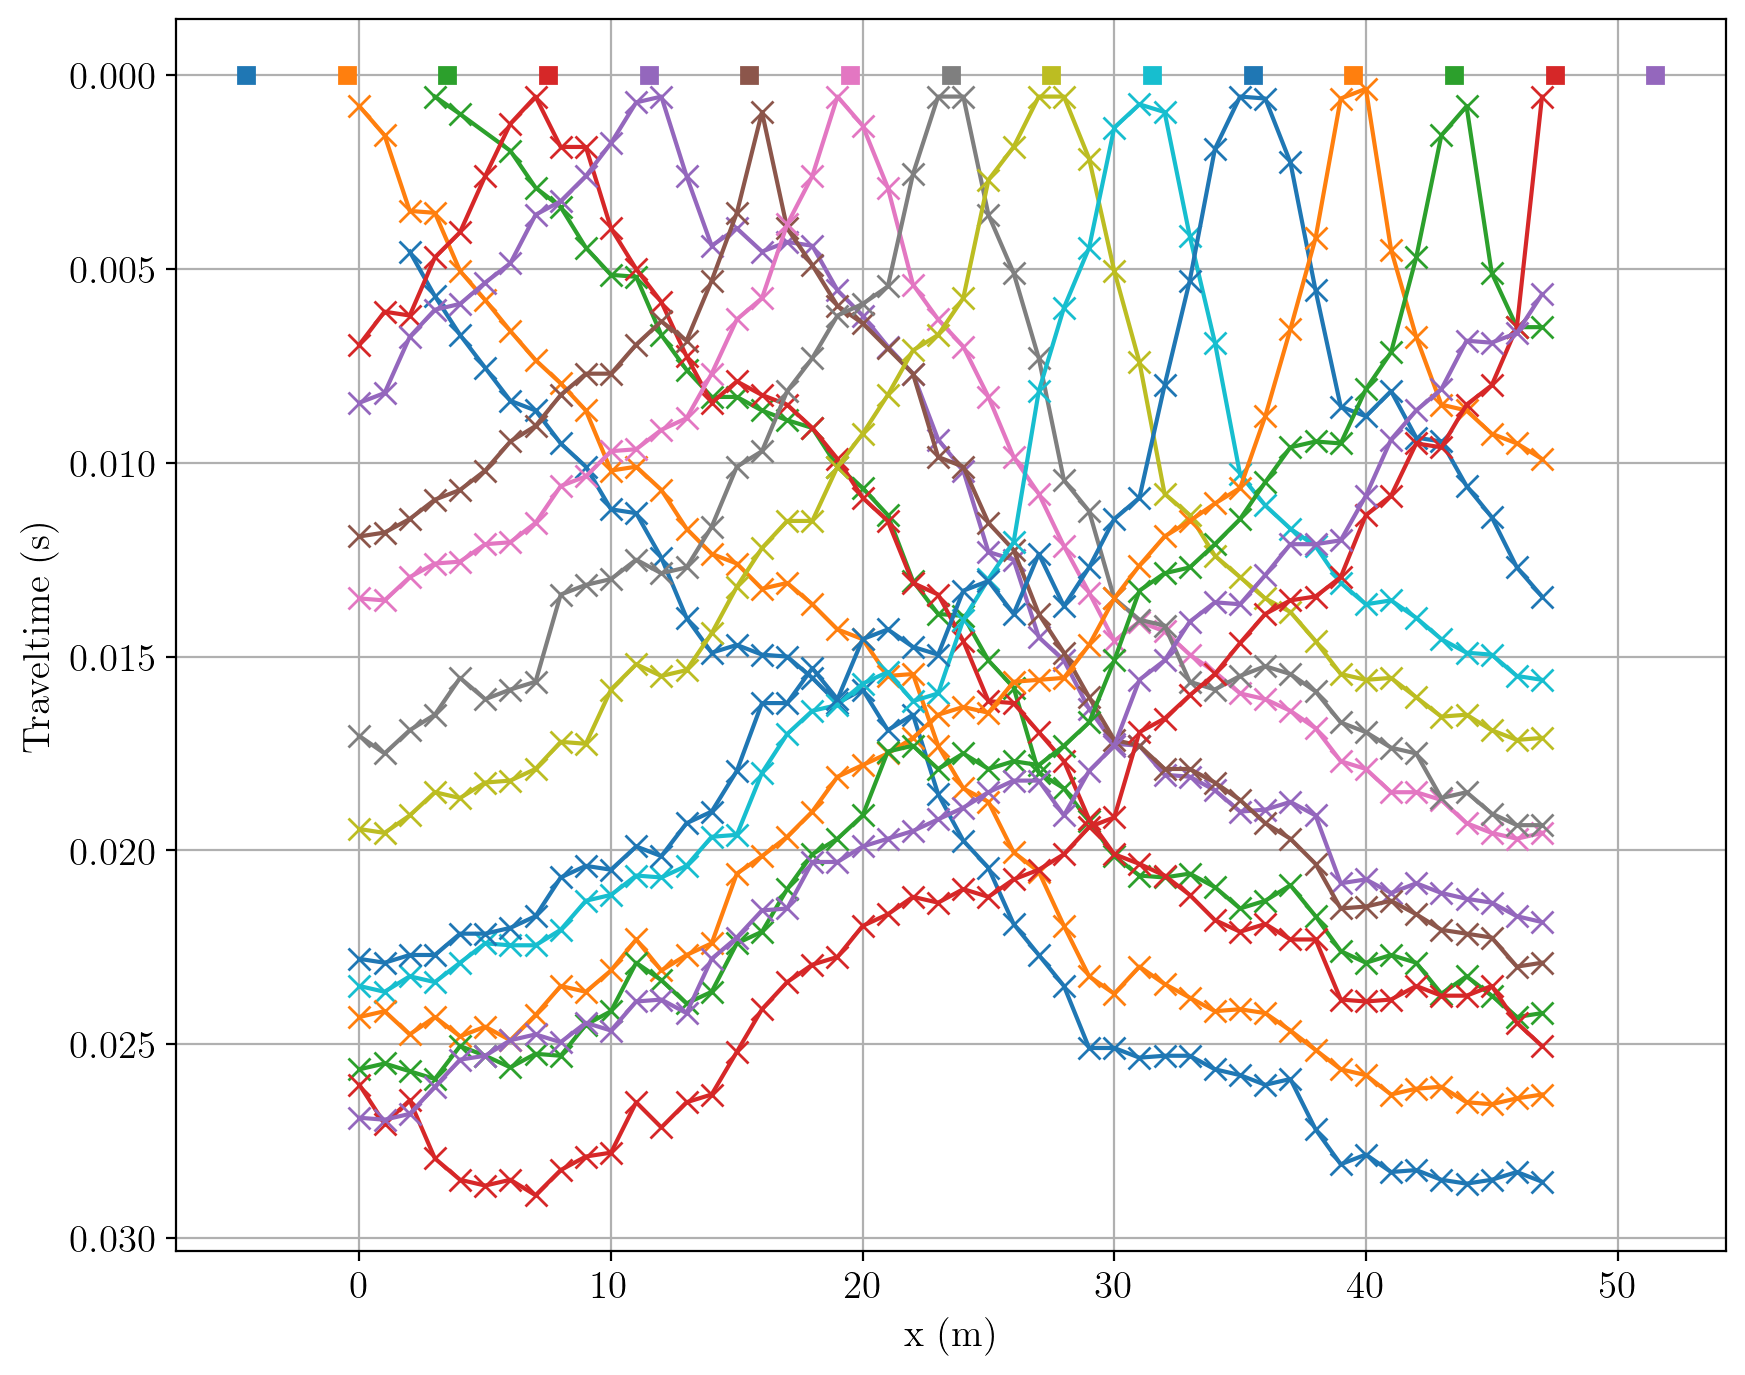
\includegraphics[width=\textwidth]{Media/p2/8.png}
\end{minipage}
\hfill
\begin{minipage}[t]{0.48\textwidth}
    \centering
    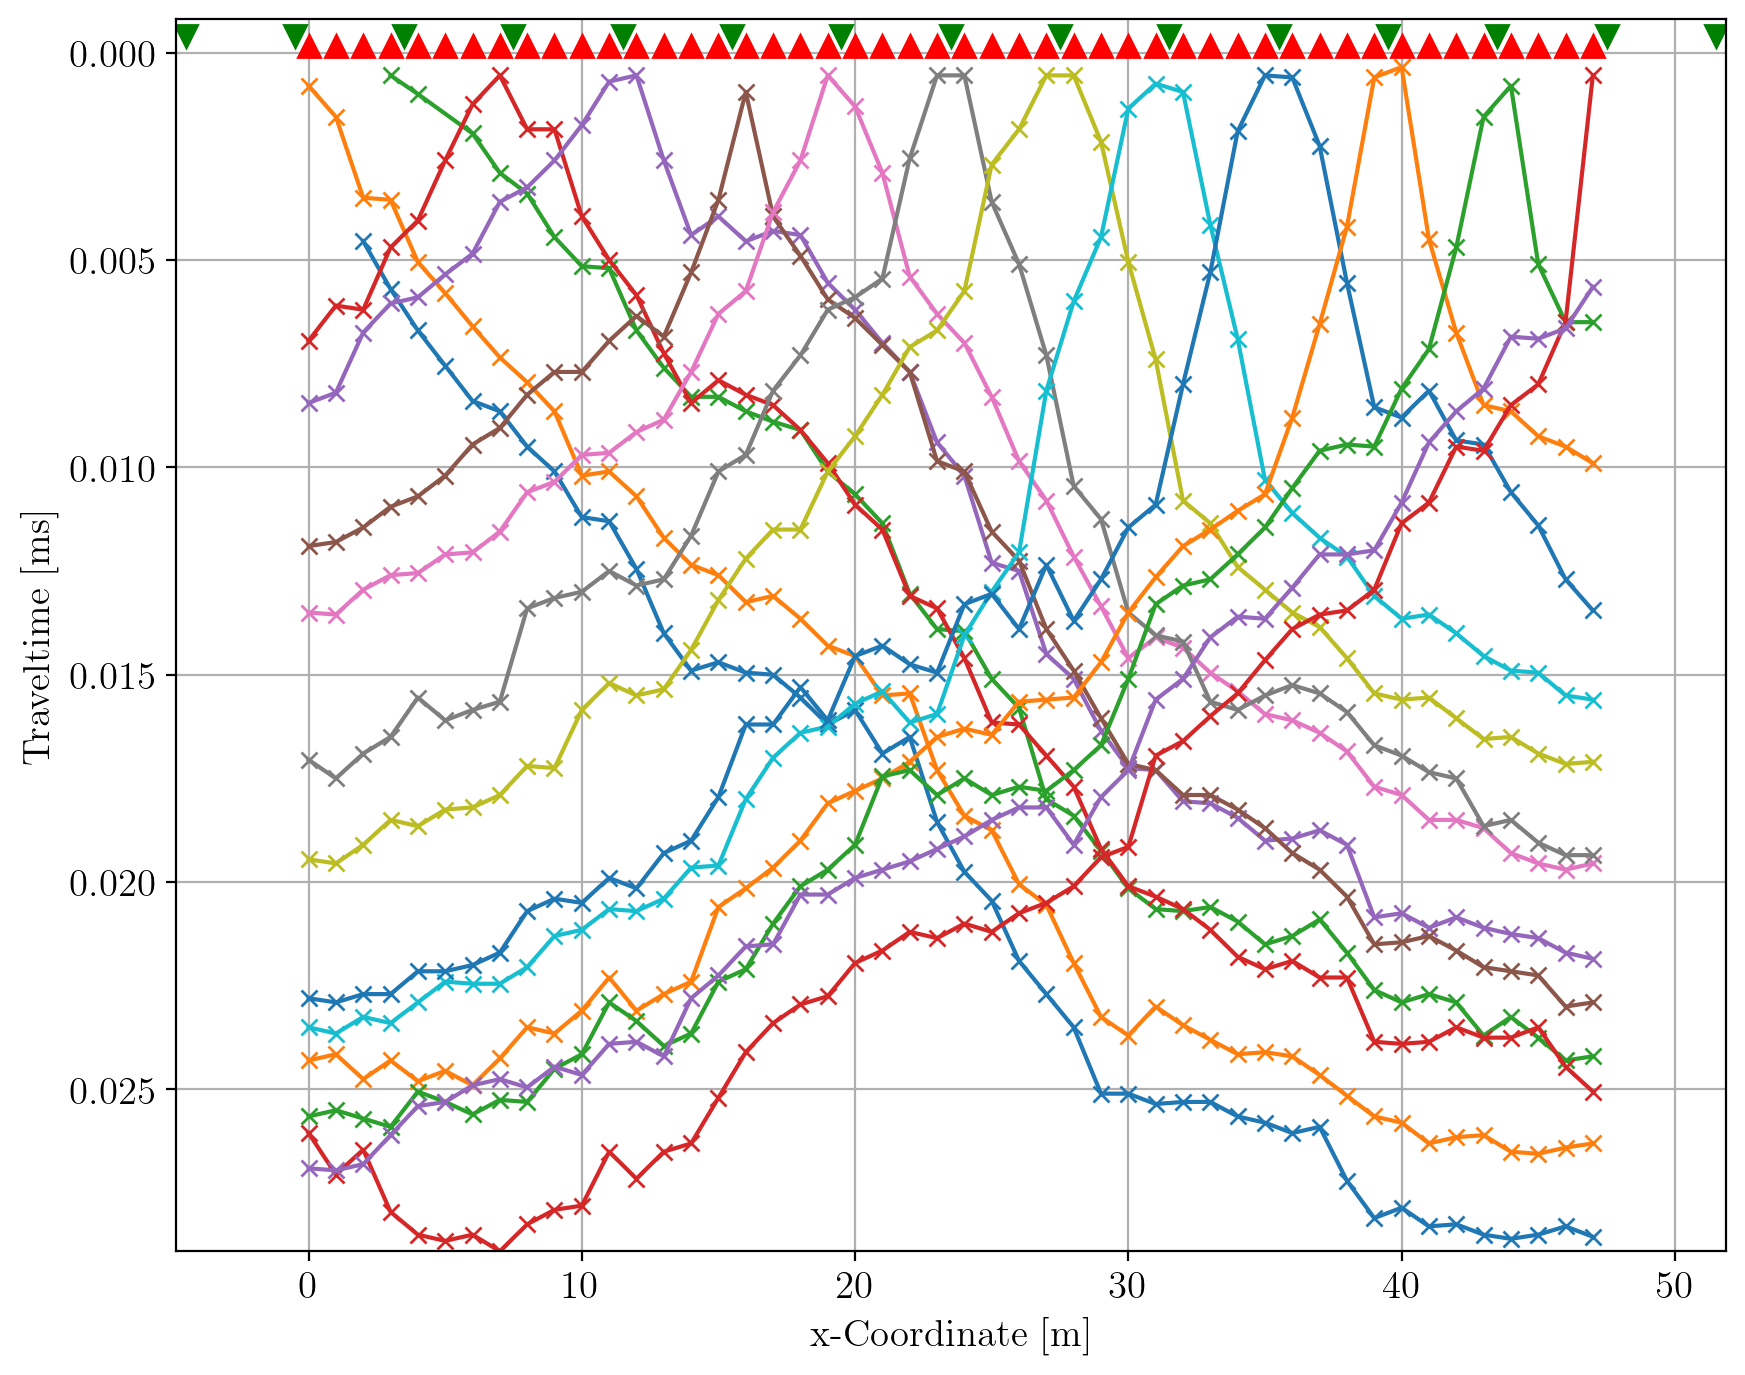
\includegraphics[width=\textwidth]{Media/p2/9.png}
\end{minipage}
\caption{(a.) First-arrival travel-time curves for the Koenigsee dataset. Each curve represents a different shot position. (b.) The same travel-time curves with {\color{ForestGreen}\textbf{green}} triangles representing the \textbf{shot} indices and {\color{red}\textbf{red}} pyramids representing the \textbf{geophone} indices.}
\end{figure}

\subsection*{Apparent Velocity Display}

An alternative visualization uses apparent velocities $v_{\text{app}}$ arranged in a matrix format with shot positions on one axis and geophone positions on the other axis, with color indicating apparent velocity magnitude:

\begin{equation}
v_{\text{app}} = \frac{\Delta x}{\Delta t} = \frac{|x_g - x_s|}{t(x_s, x_g)}
\end{equation}
This matrix representation is particularly useful for identifying data gaps and acquisition coverage, anomalous velocities indicating structural features, and quality of data (noisy vs. clear picks)

\begin{figure}[H]
\centering
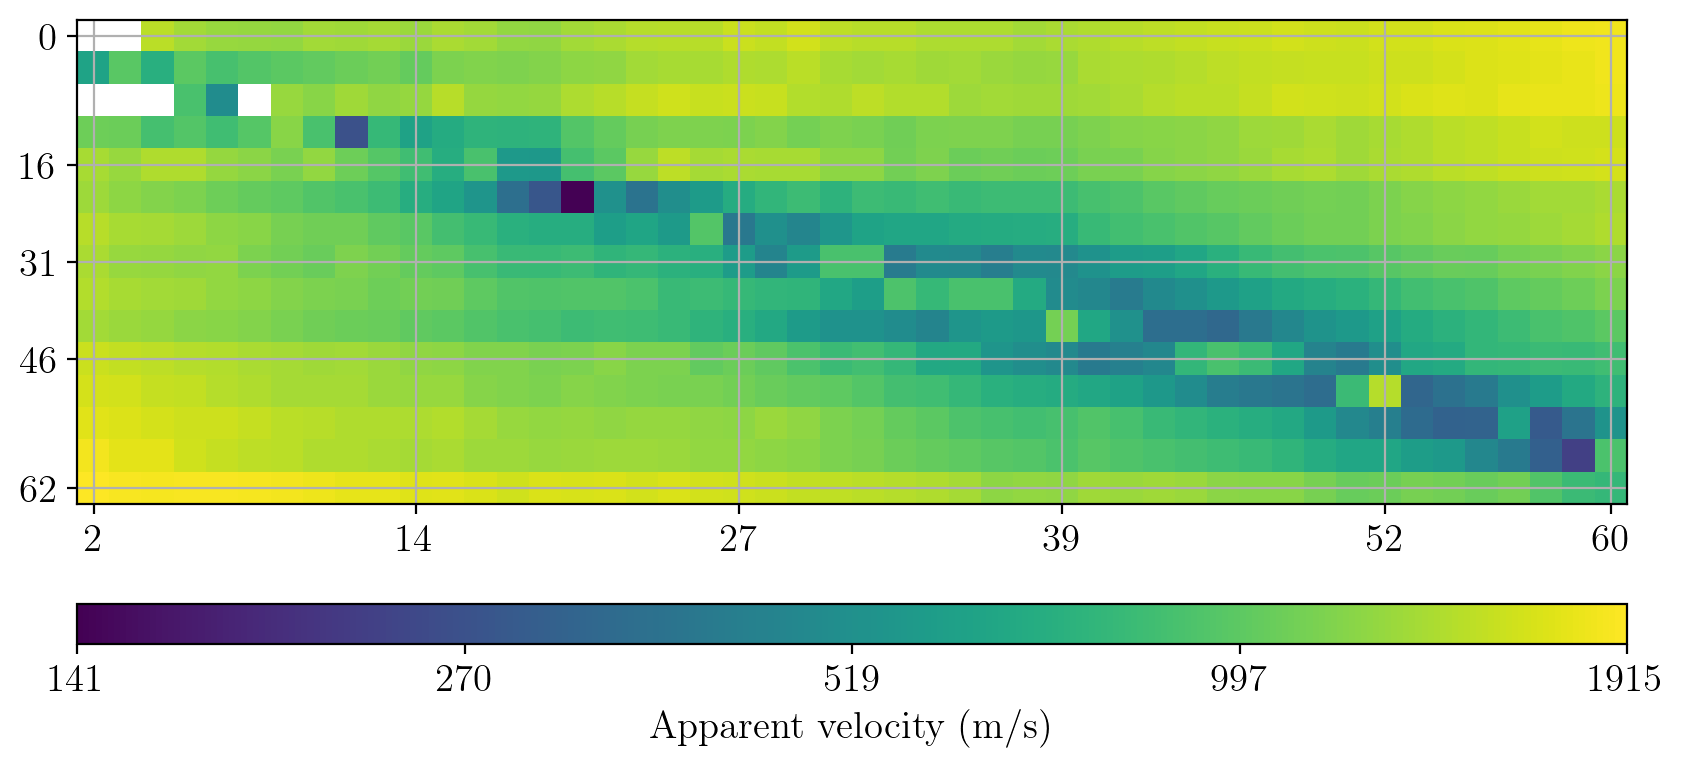
\includegraphics[width=0.9\textwidth]{Media/p2/10.png}
\caption{Apparent velocity matrix plot of the Koenigsee dataset. Shot positions are plotted on the horizontal axis, geophone positions on the vertical axis. Color scale represents apparent velocity (m/s). The visualization reveals systematic velocity variations reflecting subsurface structure and heterogeneity.}
\label{fig:apparent_velocity}
\end{figure}

\subsection*{Inversion Parameters for Koenigsee}

The Koenigsee dataset is inverted using the following parameters:

\begin{table}[H]
\centering
\caption{Inversion parameters for Koenigsee dataset}
\label{tab:inversion_params}
\begin{tabular}{|l|l|l|}
\hline
\textbf{Parameter} & \textbf{Value} & \textbf{Description} \\
\hline
\texttt{secNodes} & 3 & Secondary mesh nodes (refinement level) \\
\texttt{paraMaxCellSize} & 5.0 m & Maximum parametrization cell size \\
\texttt{zWeight} & 0.2 & Vertical weighting (anisotropic smoothness) \\
\texttt{vTop} & 500 m/s & Starting velocity at surface \\
\texttt{vBottom} & 5000 m/s & Starting velocity at depth \\
$\lambda$ & 20 & Damping Factor for regularization $\chi^2_{\text{total}} = \chi^2_{\text{data}} + \lambda \cdot R(\mathbf{m})$ \\
\hline
\end{tabular}
\end{table}

\subsection*{Parameter Interpretation}

\subsubsection*{vTop and vBottom}

PyGIMLi internally creates a \textbf{linear model} when calling \texttt{mgr.invert(.., vTop=500, vBottom=5000, ..)}. The linear gradient starting model is hence:
\begin{equation}
v_{\text{ref}}(z) = v_{\text{top}} + (v_{\text{bottom}} - v_{\text{top}}) \frac{z}{z_{\text{max}}}
\end{equation}

\subsection*{Final Inversion Map}
Final results are available at \href{https://github.com/guntas-13/travel-time-tomography/tree/master/data/TravelTimeManager}{\texttt{travel-time-tomography/data/TravelTimeManager}}.
\begin{figure}[H]
\centering
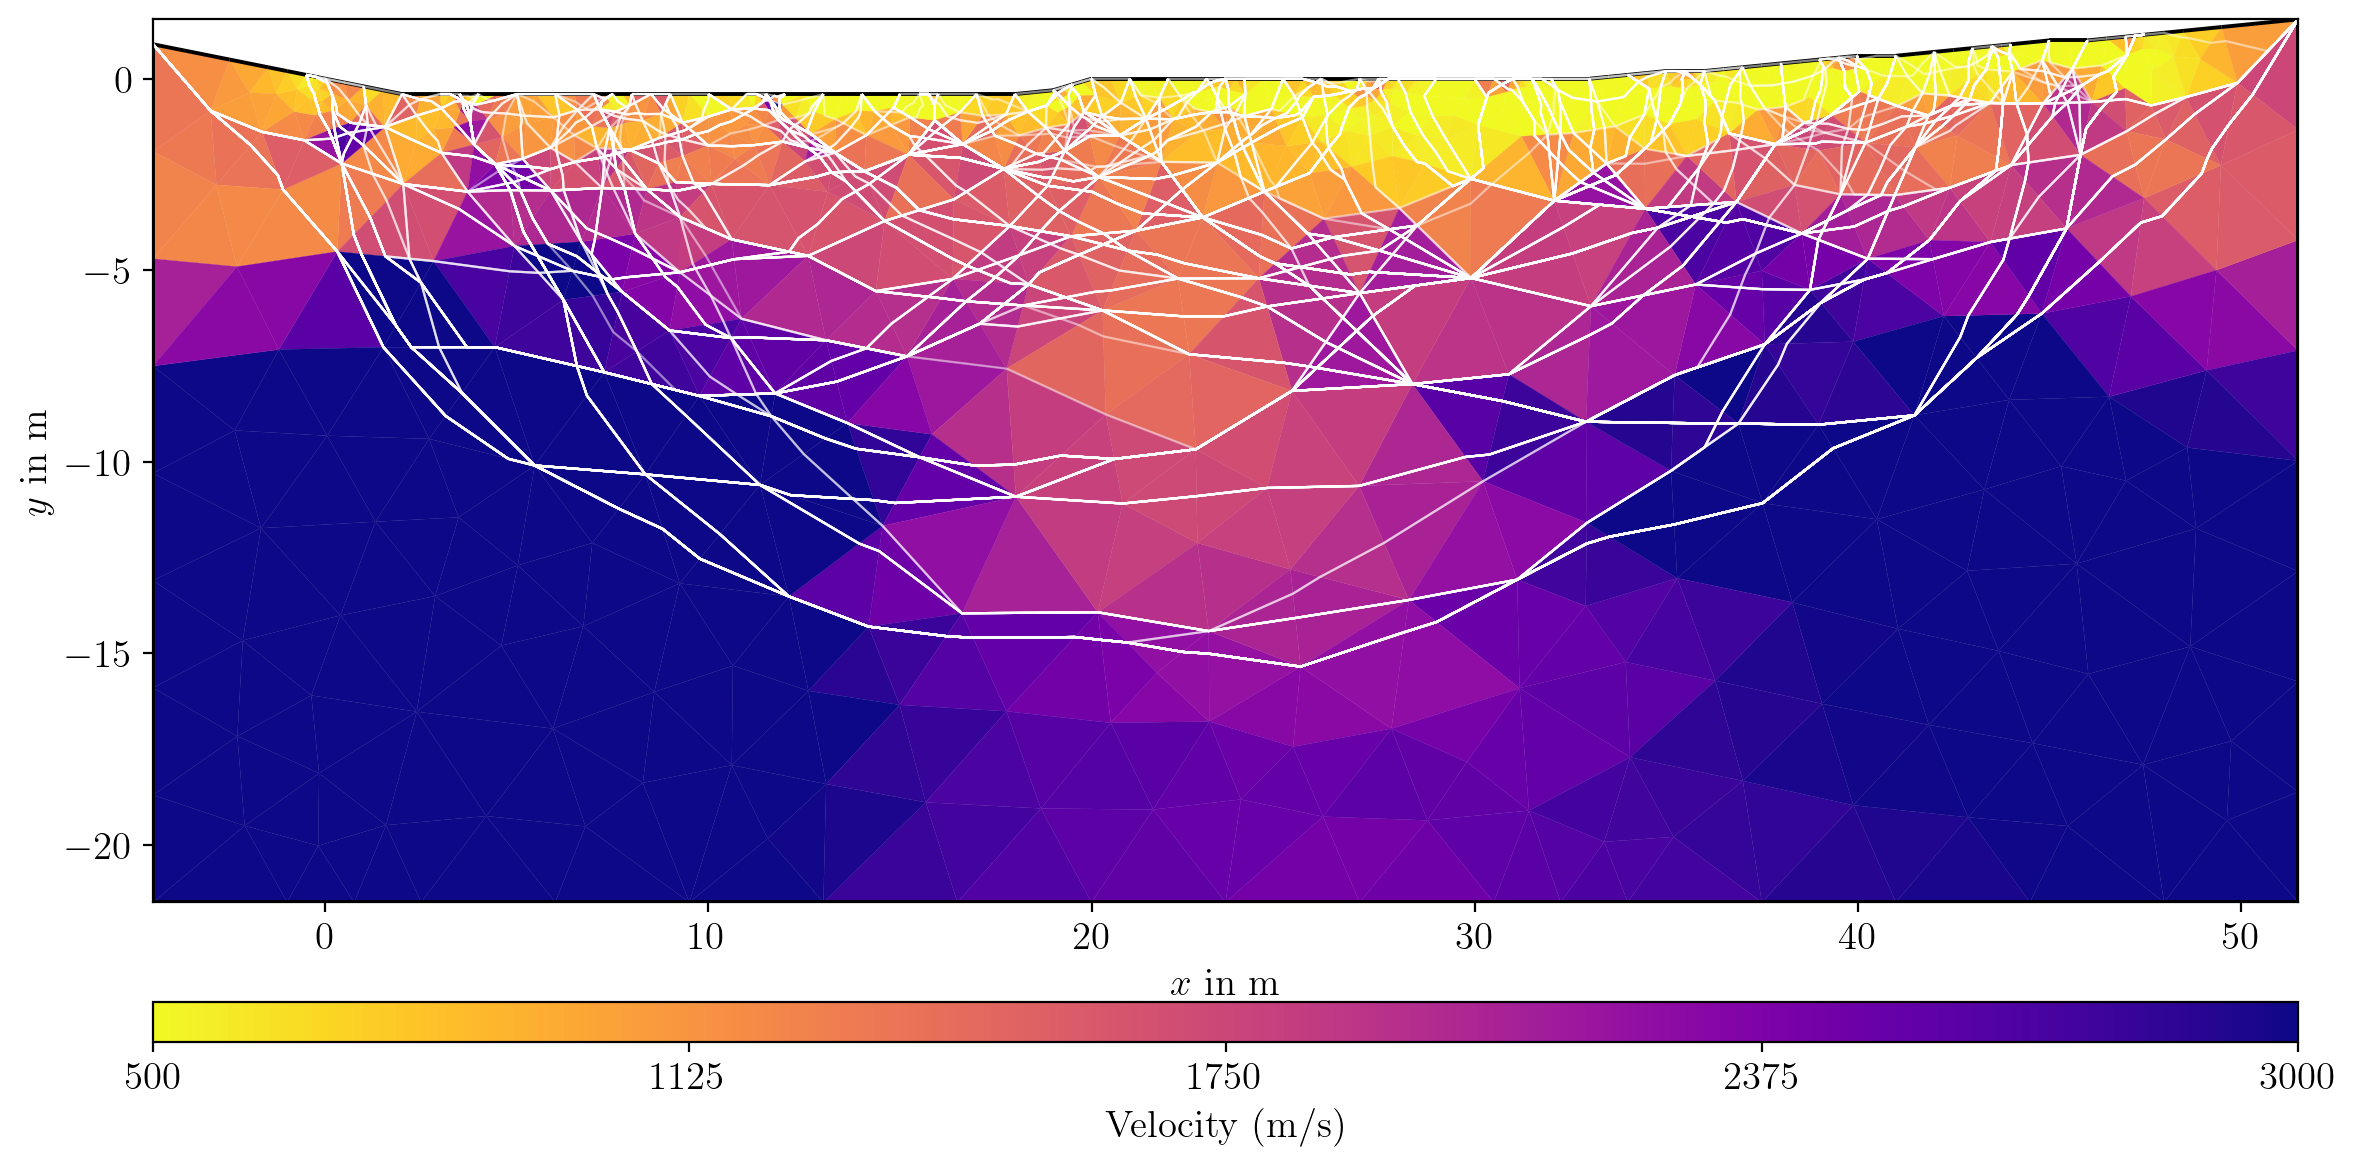
\includegraphics[width=\textwidth]{Media/p2/12.png}
% \caption{Final inverted velocity model for Koenigsee dataset. Color scale represents seismic P-wave velocity in m/s. The model reveals a three-layered structure: upper low-velocity layer (500–1200 m/s) representing weathered zone, intermediate moderate-velocity layer (1200–2000 m/s), and high-velocity bedrock (2000–2693 m/s). Superimposed ray coverage (or ray paths) indicates illumination of the model by the seismic ray paths}
\caption{Final inverted velocity model for Koenigsee dataset. Color scale shows seismic P-wave velocity (m/s). The result reveals a broad U-shaped low-velocity zone flanked by higher-velocity regions, consistent with basinal infill above deeper bedrock, rather than a horizontally stratified or simply layered profile. Superimposed ray coverage (or ray paths) indicates region-specific illumination by the data.}
\end{figure}

\begin{figure}[H]
\centering
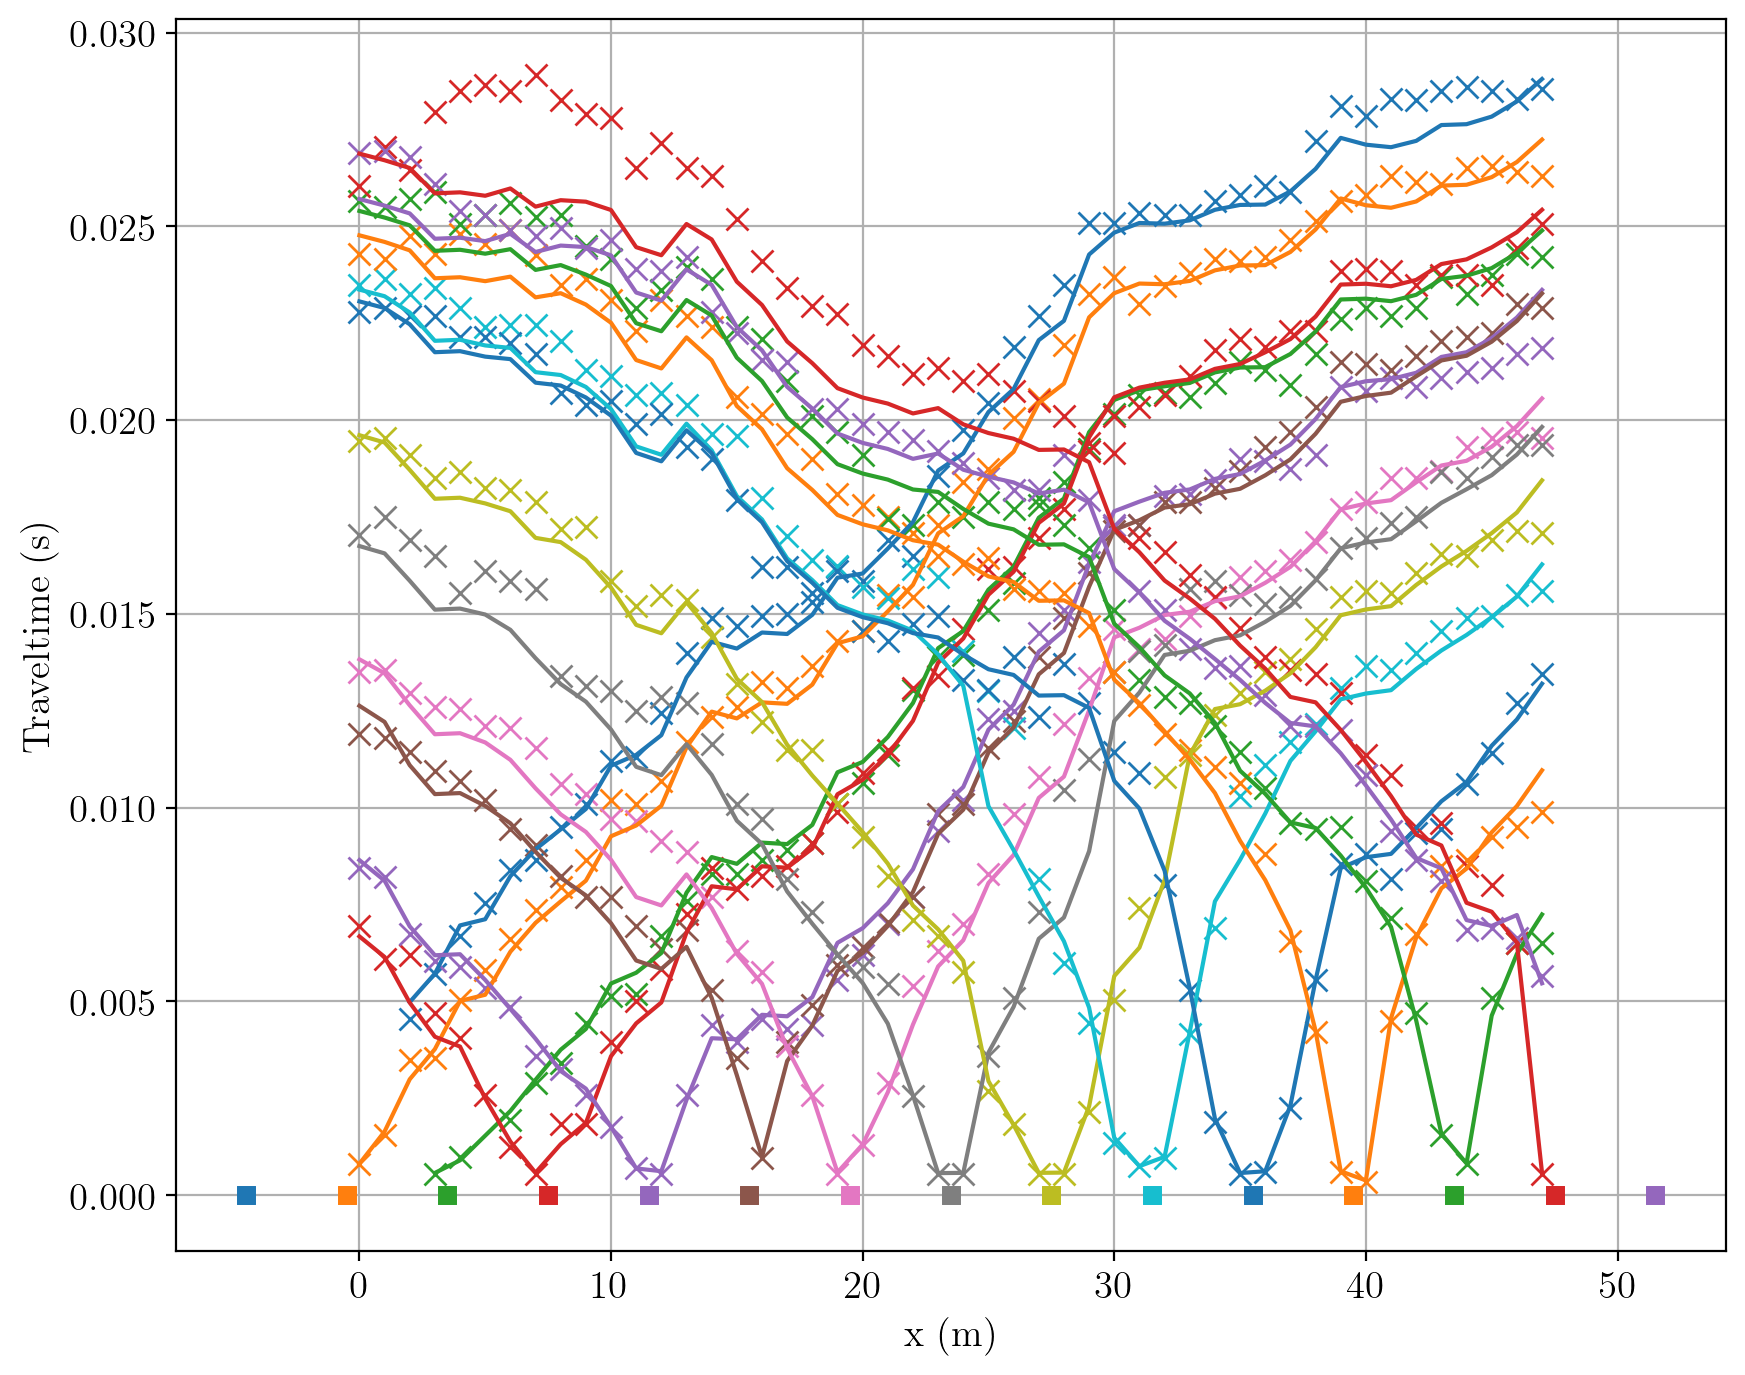
\includegraphics[width=\textwidth]{Media/p2/11.png}
\caption{The corresponding predicted travel-time arrival data calculated using the inverted velocity model through forward ray tracing indicating
residual misfit.}
\end{figure}

\bigskip
\hrule

\newpage
\section*{Modelling a Synthetic 2D Crosshole Tomography}
\begin{figure}[H]
\centering
\begin{minipage}[t]{0.48\textwidth}
    \centering
    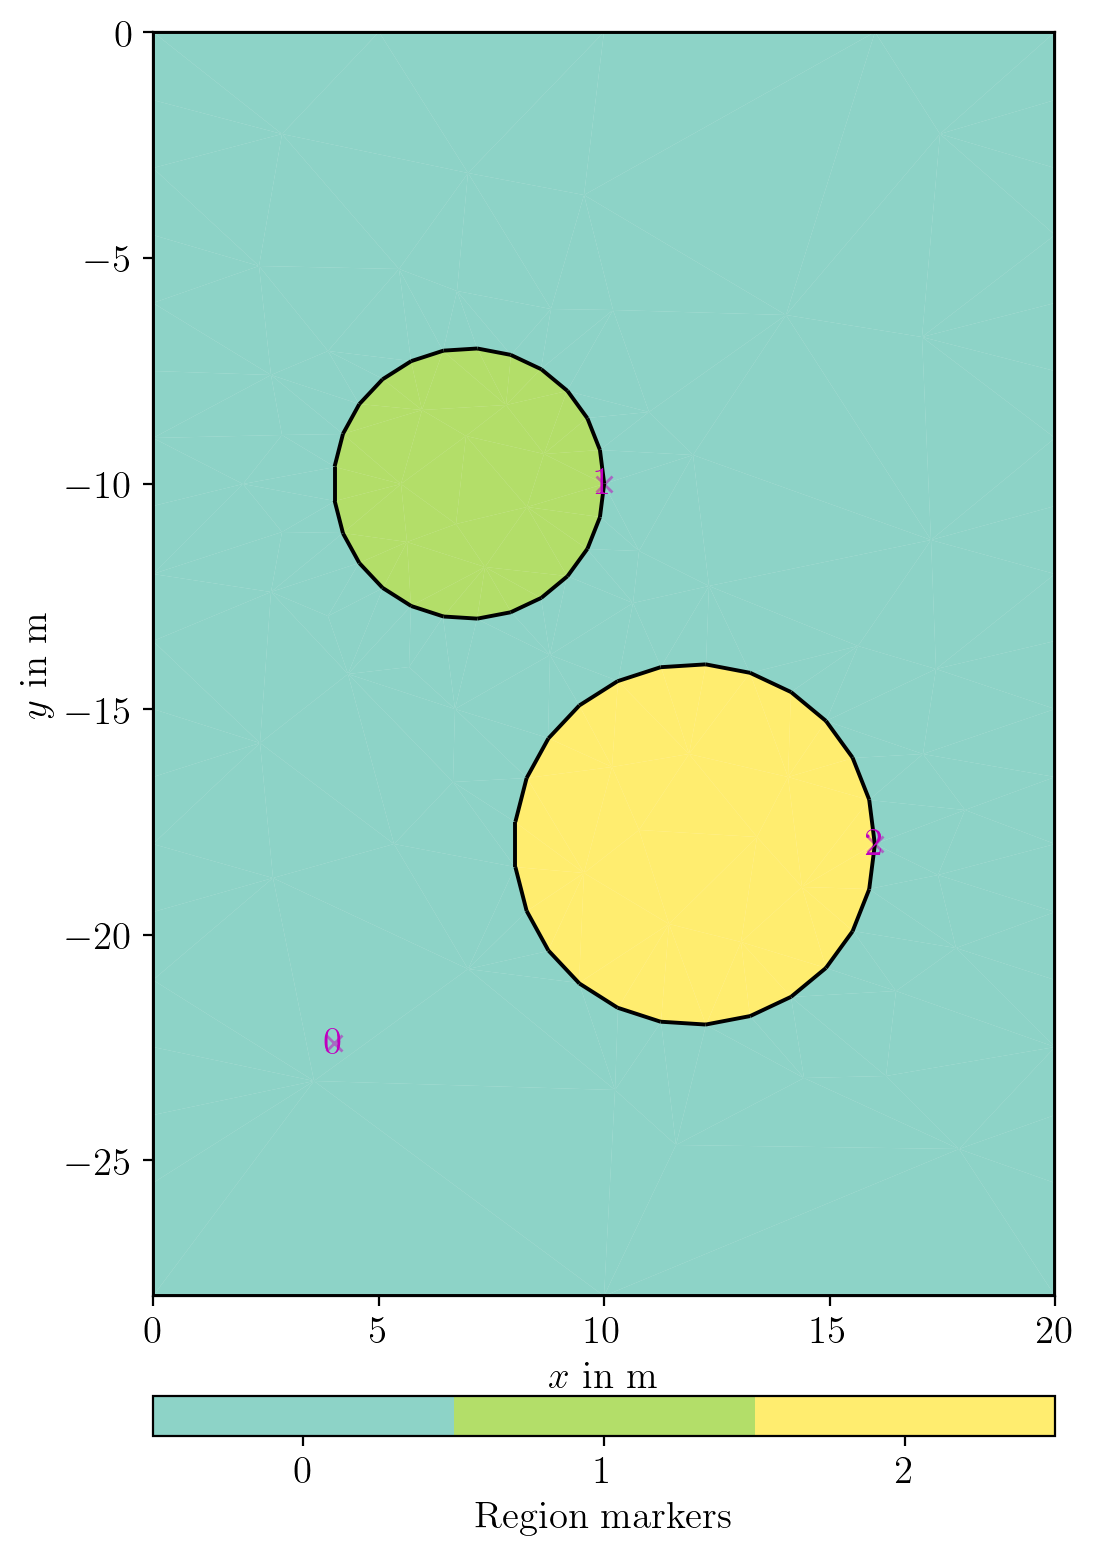
\includegraphics[width=\textwidth]{Media/p3/13.png}
\end{minipage}
\hfill
\begin{minipage}[t]{0.48\textwidth}
    \centering
    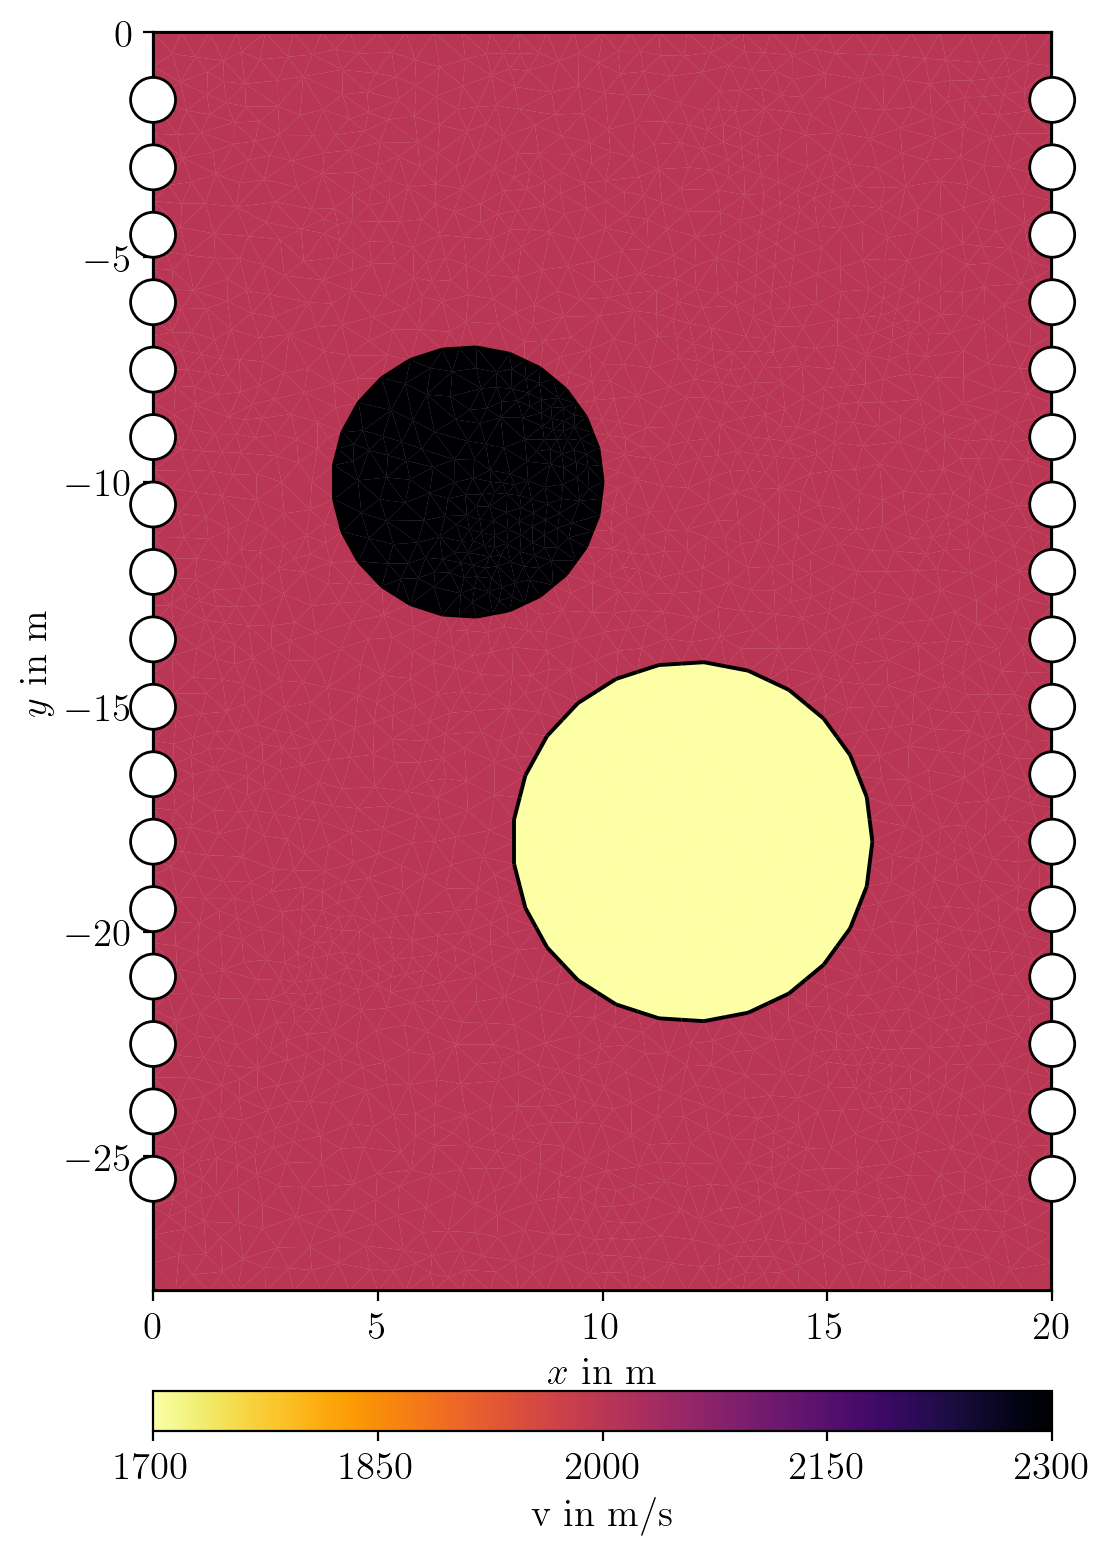
\includegraphics[width=\textwidth]{Media/p3/16.png}
\end{minipage}
\caption{(a.) Schematic of the survey geometry. (b.) True synthetic velocity model showing background (2000 m/s), high-velocity anomaly (2300 m/s) at (7, -10) m, and low-velocity anomaly (1700 m/s) at (12, -18) m along with crosshole geometry: two boreholes separated by 20 m, with 17 sensors per borehole.}
\label{fig:crosshole_geometry}
\end{figure}

\subsection*{Objective}
Demonstrate the modelling of traveltimes and their inversion for the underlying slowness distribution for a crosshole scenario.

\subsection*{Borehole Configuration}
Two vertical boreholes are deployed in a shallow subsurface domain. Geophones are deployed at regular vertical intervals in both boreholes. All shots are deployed at every sensor position in Borehole A; all sensors in Borehole B act as receivers. Ray paths connect every shot-receiver pair horizontally between boreholes, with vertical offset determined by sensor depth differences. Unlike surface refraction (where rays propagate down and back up), crosshole rays propagate primarily horizontally.
\begin{table}[H]
\small
\centering
\caption{Crosshole acquisition parameters}
\label{tab:crosshole_acquisition}
\begin{tabular}{|l|c|}
\hline
\textbf{Parameter} & \textbf{Value} \\
\hline
Horizontal borehole spacing & \texttt{20.0 m} \\
Sensor spacing (vertical) & \texttt{1.5 m} \\
No. of sensors & \texttt{34} \\
Domain & \texttt{[0, 20] m (x) $\times$ [0, -28] m (z)} \\
\hline
\end{tabular}
\end{table}

\subsection*{True Velocity Model and Parameterization}

The true velocity model consists of:

\begin{itemize}
    \item \textbf{Background velocity}: $v_{\text{bg}} = 2000$ m/s throughout the domain $[0, 20] \times [0, -25]$ m (marker 1)
    \item \textbf{Low-velocity anomaly}: A circular region centered at $(x, z) = (7.0, -10.0)$ m with radius 3 m, velocity $v_{\text{low}} = 1700$ m/s (marker 2)
    \item \textbf{High-velocity anomaly}: A circular region centered at $(x, z) = (12.0, -18.0)$ m with radius 4 m, velocity $v_{\text{high}} = 2300$ m/s (marker 3)
\end{itemize}

The velocity distribution is:
\begin{equation}
v(\mathbf{r}) = \begin{cases}
2000 \text{ m/s} & \text{background} \\
1700 \text{ m/s} & \text{low-velocity anomaly} \\
2300 \text{ m/s} & \text{high-velocity anomaly}
\end{cases}
\end{equation}

\subsection*{Forward Modelling: Synthetic data generation}
\begin{itemize}
  \item Forward simulation call:
  \texttt{tt.simulate(mesh=mesh\_fwd, scheme=scheme, slowness=1./model, secNodes=4, noiseLevel=0.001, noiseAbs=1e-5, seed=1337)}.
  \item Noise: relative noise = 0.1\% (\texttt{noiseLevel=0.001}), absolute noise = 10 $\mu s$, seed fixed for reproducibility.
\end{itemize}
\begin{figure}[H]
\centering
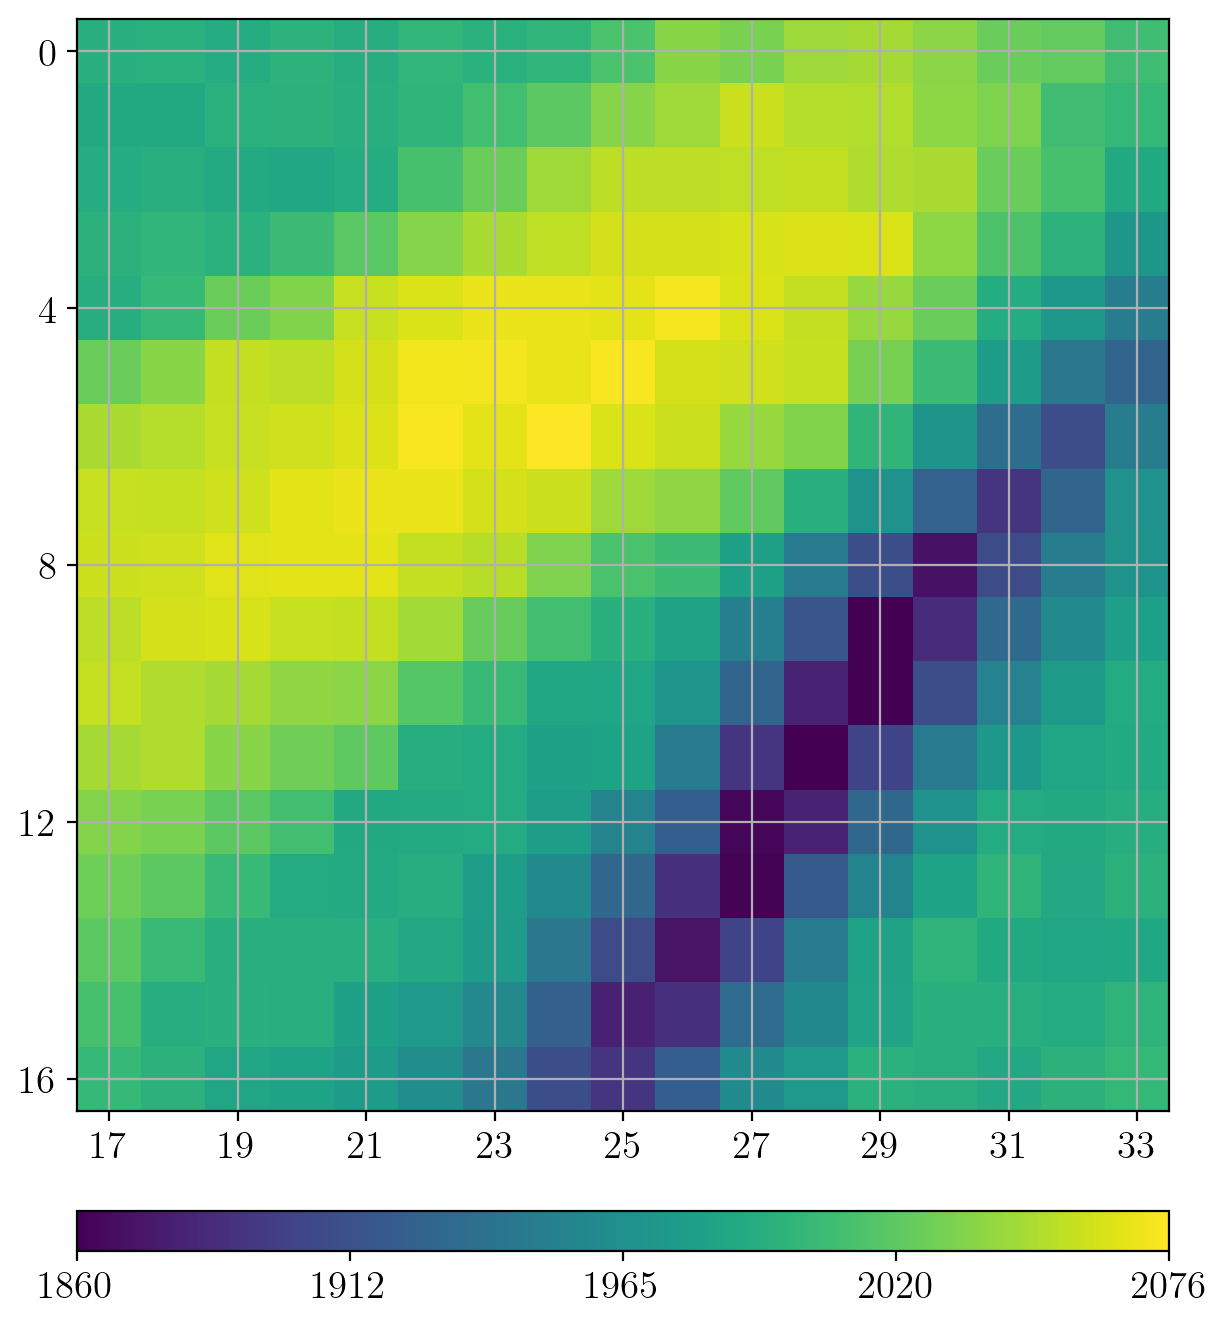
\includegraphics[width=0.5\textwidth]{Media/p3/17.png}
\caption{Apparent velocity matrix plot. Shot positions are plotted on the horizontal axis, geophone positions on the vertical axis. Color scale represents apparent velocity (m/s). The visualization reveals systematic velocity variations reflecting subsurface structure and heterogeneity.}
\end{figure}


\subsubsection*{Dijkstra Ray-Tracing Operator}

PyGIMLi creates a \textbf{TravelTimeDijkstraModelling} forward operator takes a velocity model $\mathbf{m}$, converts velocity to slowness: $s = 1/v$, traces rays from each shot to each receiver using Dijkstra's algorithm, returns predicted travel times $\mathbf{d}_{\text{pred}} = \mathbf{f}(\mathbf{m})$

\subsubsection*{How Dijkstra Ray Tracing Works}
Dijkstra's algorithm solves the \textbf{eikonal equation} numerically:
\begin{equation}
|\nabla T(\mathbf{r})|^2 = \frac{1}{v^2(\mathbf{r})}
\end{equation}
\textbf{Algorithm steps}:
\begin{enumerate}
    \item Initialize travel-time field $T$ to infinity everywhere except at the source: $T(\text{source}) = 0$
    \item Build a directed graph where:
    \begin{itemize}
        \item Nodes = mesh vertices
        \item Edges connect adjacent nodes
        \item Edge weight = distance $/ v_{\text{avg}}$ (slowness-weighted distance)
    \end{itemize}
    \item Use Dijkstra's shortest-path algorithm to compute minimum travel times to all receivers
\end{enumerate}

\textbf{Computational complexity}: $O(n \log n)$ where $n$ is the number of mesh nodes
\subsection*{Inversion Problem}
The inverse problem seeks to recover the velocity model $\mathbf{m}$ from observed travel times $\mathbf{d}_{\text{obs}}$ by minimizing the misfit functional:

\begin{equation}
\chi^2(\mathbf{m}) = \sum_{i=1}^{N_{\text{data}}} \left( \frac{T_i(\mathbf{m}) - d_i^{\text{obs}}}{\sigma_i} \right)^2 + \lambda \, R(\mathbf{m})
\end{equation}

where:
\begin{itemize}
    \item $T_i(\mathbf{m})$ = predicted travel time for ray $i$ in model $\mathbf{m}$
    \item $d_i^{\text{obs}}$ = observed travel time for ray $i$
    \item $\sigma_i$ = measurement uncertainty for ray $i$
    \item $R(\mathbf{m})$ = regularization functional (smoothness constraint)
    \item $\lambda$ = regularization parameter (trade-off between data fit and model smoothness)
\end{itemize}
The velocity model is parameterized on a finite element mesh with velocity values at cell centers or vertices:
\begin{equation}
\mathbf{m} = [v_1, v_2, \ldots, v_{N_{\text{cells}}}]^T
\end{equation}
For inversion purposes, velocities are typically transformed to \textbf{logarithmic slowness}:
\begin{equation}
\mathbf{m}_{\text{slow}} = [\log(s_1), \log(s_2), \ldots, \log(s_{N_{\text{cells}}})]^T
\end{equation}

\subsection*{Regularization Strategy}

PyGIMLi automatically sets up \textbf{Tikhonov regularization}. The regularization term enforces smoothness and helps stabilize the inverse solution:

\begin{equation}
R(\mathbf{m}) = \int_{\Omega} \left( w_z^2 |\partial_z \mathbf{m}|^2 + |\partial_x \mathbf{m}|^2 \right) d\Omega + \alpha |\mathbf{m} - \mathbf{m}_{\text{ref}}|^2
\end{equation}
where $\mathbf{m}_{\text{ref}}$ is a reference model and $\alpha$ controls the coupling to the reference model.

\subsection*{Iterative Inversion Steps}

The inversion is typically performed using an iterative Gauss-Newton or damped least-squares approach:

\begin{equation}
\mathbf{m}^{(k+1)} = \mathbf{m}^{(k)} + \left( \mathbf{J}^T \mathbf{J} + \lambda \mathbf{R} \right)^{-1} \mathbf{J}^T \left( \mathbf{d}_{\text{obs}} - \mathbf{T}(\mathbf{m}^{(k)}) \right)
\end{equation}

where $\mathbf{J}$ is the Jacobian matrix of partial derivatives of travel times with respect to model parameters.

\subsection*{Convergence Criteria}

Inversion iterations continue until convergence based on criteria such as:

\begin{itemize}
    \item Relative data misfit reduction: $\frac{\chi^2(k) - \chi^2(k+1)}{\chi^2(k)} < \varepsilon_{\text{rel}}$
    \item Absolute misfit threshold: $\chi^2(k) < \chi^2_{\text{target}}$
    \item Maximum iteration count: $k < k_{\max}$
\end{itemize}

\subsection*{Inversion Mesh \& Parameters}
\begin{figure}[H]
\centering
\begin{minipage}[t]{0.48\textwidth}
    \centering
    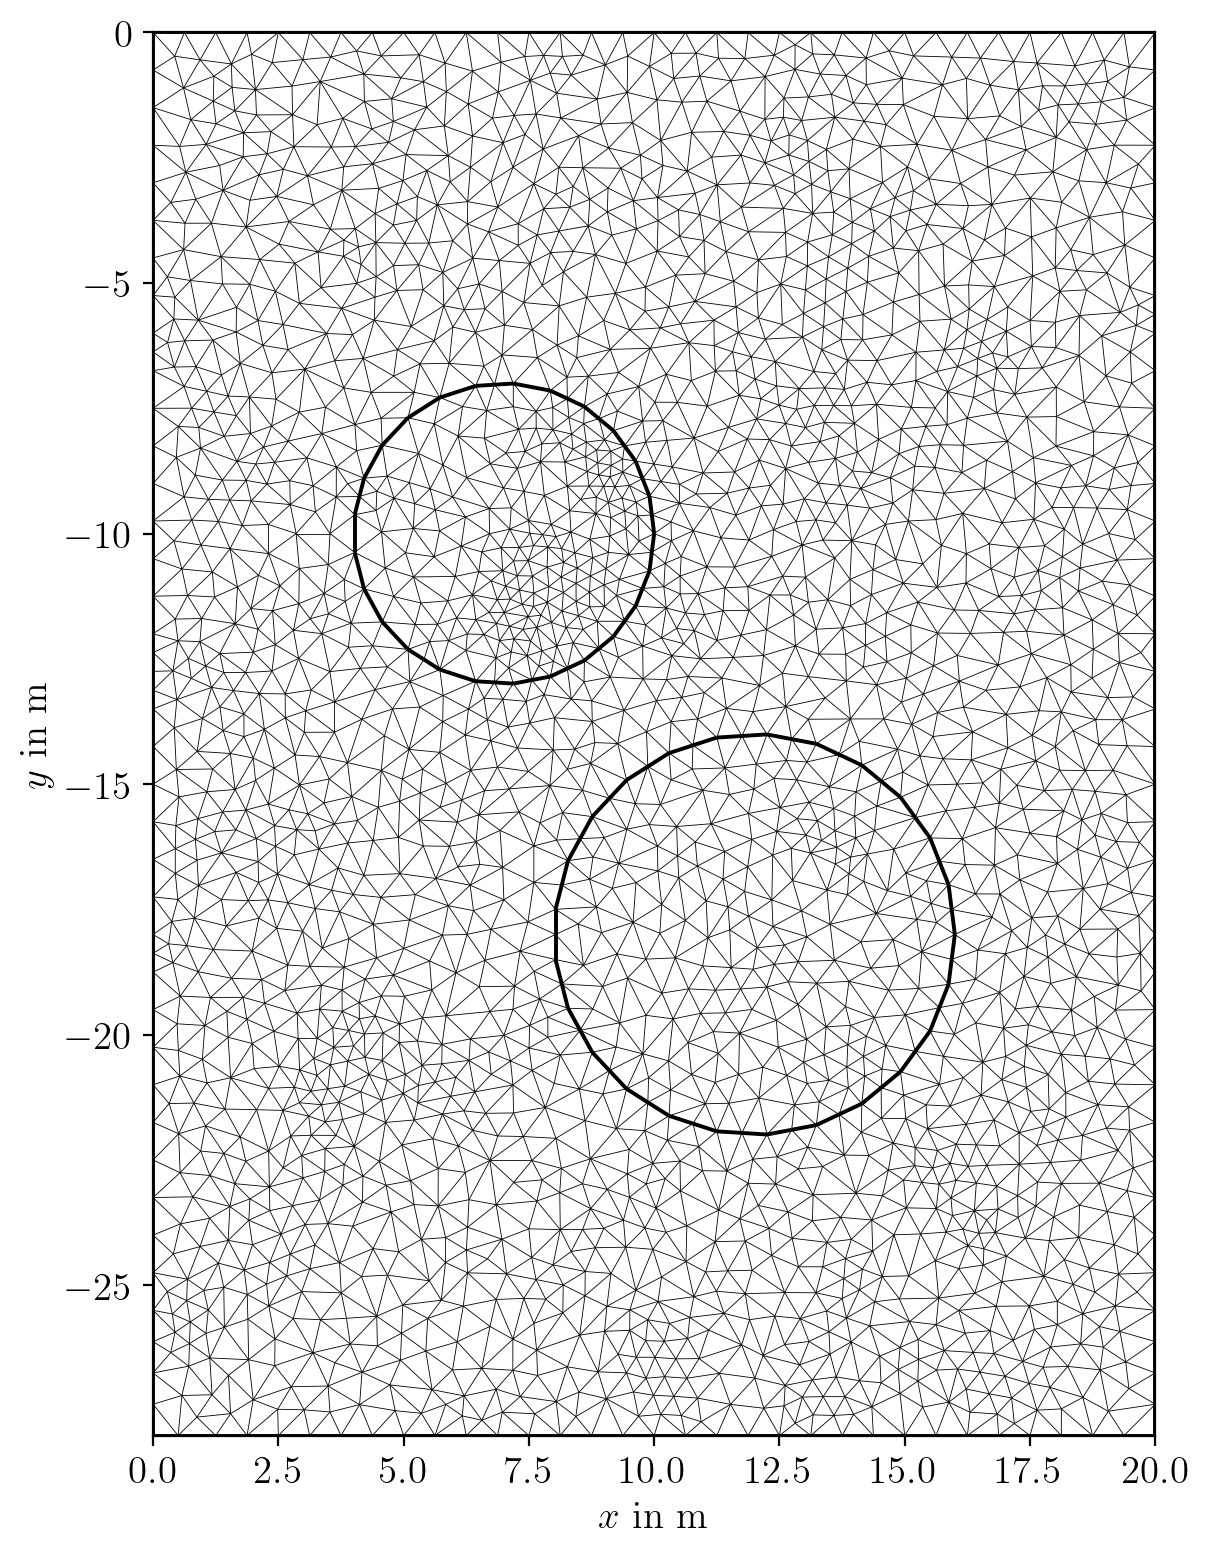
\includegraphics[width=\textwidth]{Media/p3/14.png}
\end{minipage}
\hfill
\begin{minipage}[t]{0.48\textwidth}
    \centering
    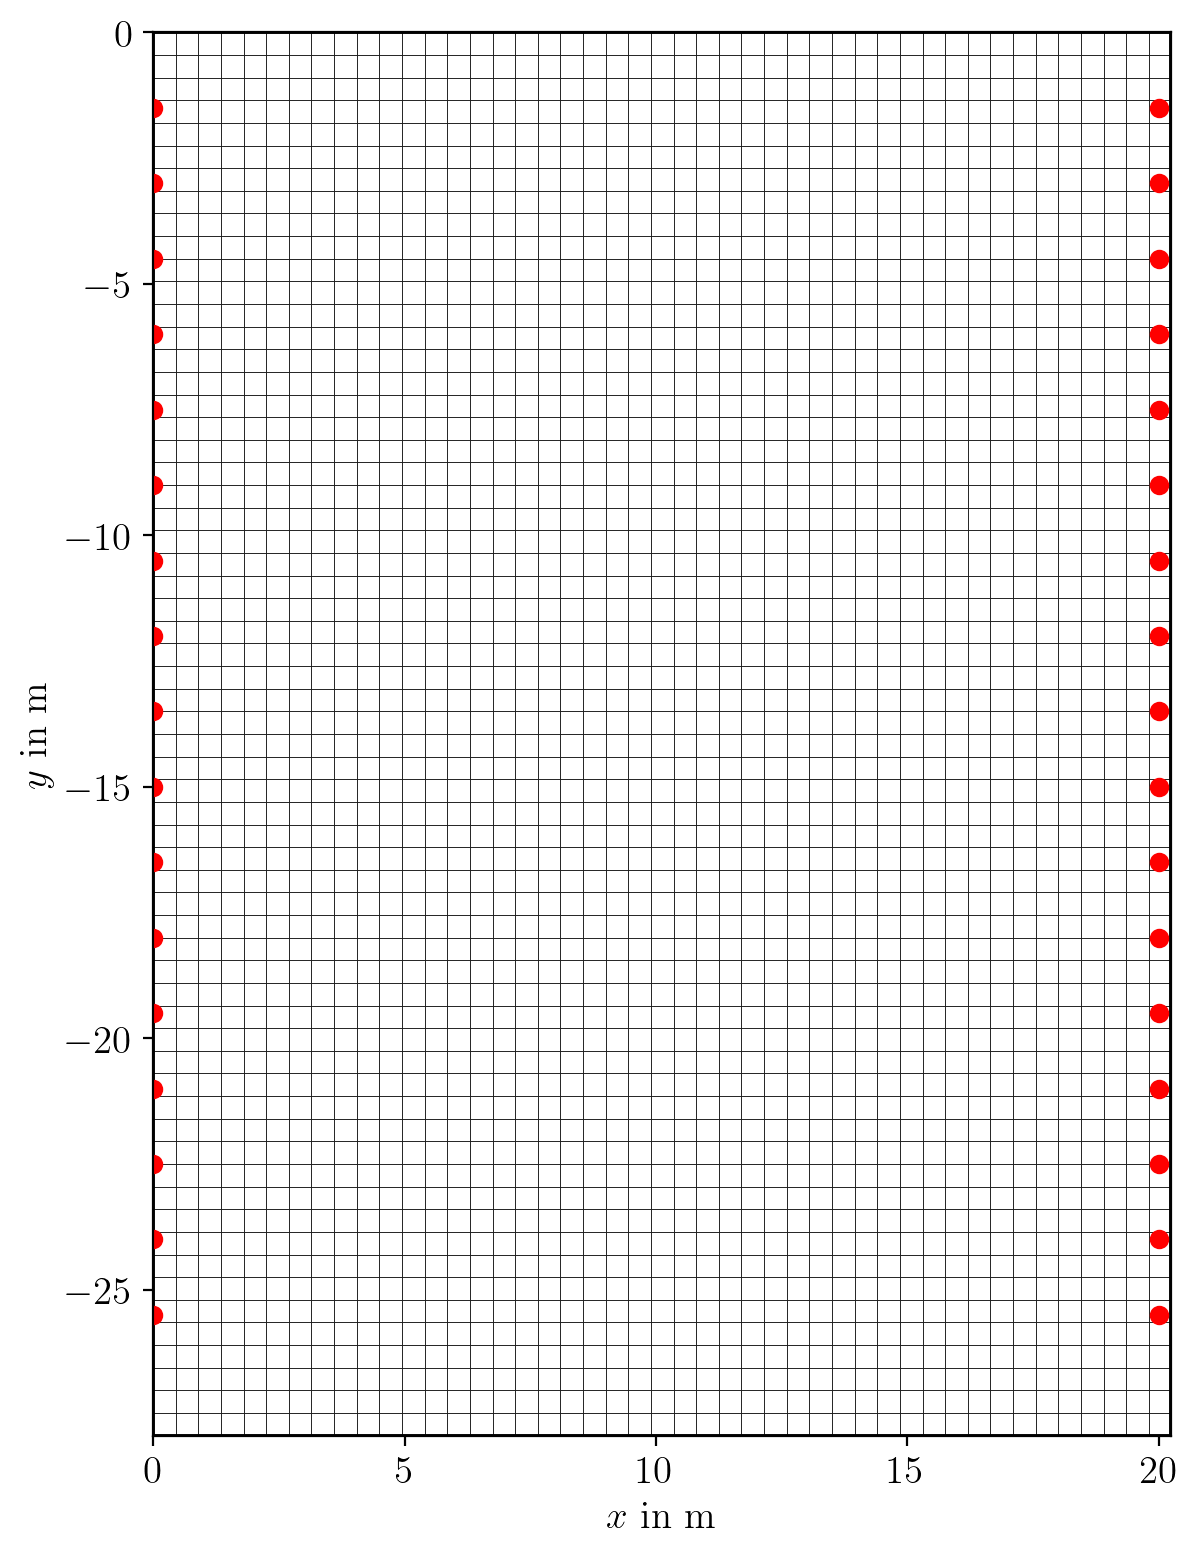
\includegraphics[width=\textwidth]{Media/p3/18.png}
\end{minipage}
\caption{(a.) Triangular mesh used for forward modelling. (b.) Coarse structured mesh used during inversion.}
\end{figure}
Rather than using the fine forward mesh for inversion, a coarser structured grid is constructed:

\begin{table}[H]
\centering
\caption{Inversion mesh specifications}
\begin{tabular}{|l|c|p{6cm}|}
\hline
\textbf{Parameter} & \textbf{Value} & \textbf{Description} \\
\hline
X-extent & \texttt{[0, 20] m} & 28 grid points \\
Y-extent & \texttt{[0, -28] m} & 39 grid points \\
Cell spacing & 0.75 m & Regular rectangular cells \\
\hline
\end{tabular}
\end{table}
Convergence stops when $\chi^2\le1$. A homogeneous starting model is used \texttt{useGradient=False}. This results in:
\begin{verbatim}
invmodel = mgr.invert(data, mesh=mesh, secNodes=3, lam=1000, 
                      zWeight=1.0, useGradient=False, 
                      verbose=True)
\end{verbatim}
\begin{align*}
v_0(\mathbf{r}) &= 2000 \text{ m/s} \quad \forall \mathbf{r} \\
s_0(\mathbf{r}) &= \frac{1}{2000} = 5.0 \times 10^{-4} \text{ s/m} \quad \forall \mathbf{r}
\end{align*}
This choice of homogeneous starting model is justified for crosshole geometry: velocity typically does NOT vary systematically with depth between boreholes, so a gradient model (appropriate for surface surveys) is not used.
\begin{table}[H]
\centering
\caption{Crosshole inversion parameters}
\begin{tabular}{|l|c|p{7cm}|}
\hline
\textbf{Parameter} & \textbf{Value} & \textbf{Description} \\
\hline
\texttt{lam} & 1000 & Strong damping/regularization parameter \\
\texttt{zWeight} & 1.0 & Isotropic smoothness \\
\texttt{useGradient} & False & Homogeneous starting model \\
Data transformation & Identity & Travel times used directly \\
Model transformation & Log-slowness & Inversion in $\mathbf{p} = \log(\mathbf{s})$ space \\
\hline
\end{tabular}
\end{table}

\subsection*{Inversion Results}

\begin{figure}[H]
\centering
\begin{minipage}[t]{0.48\textwidth}
    \centering
    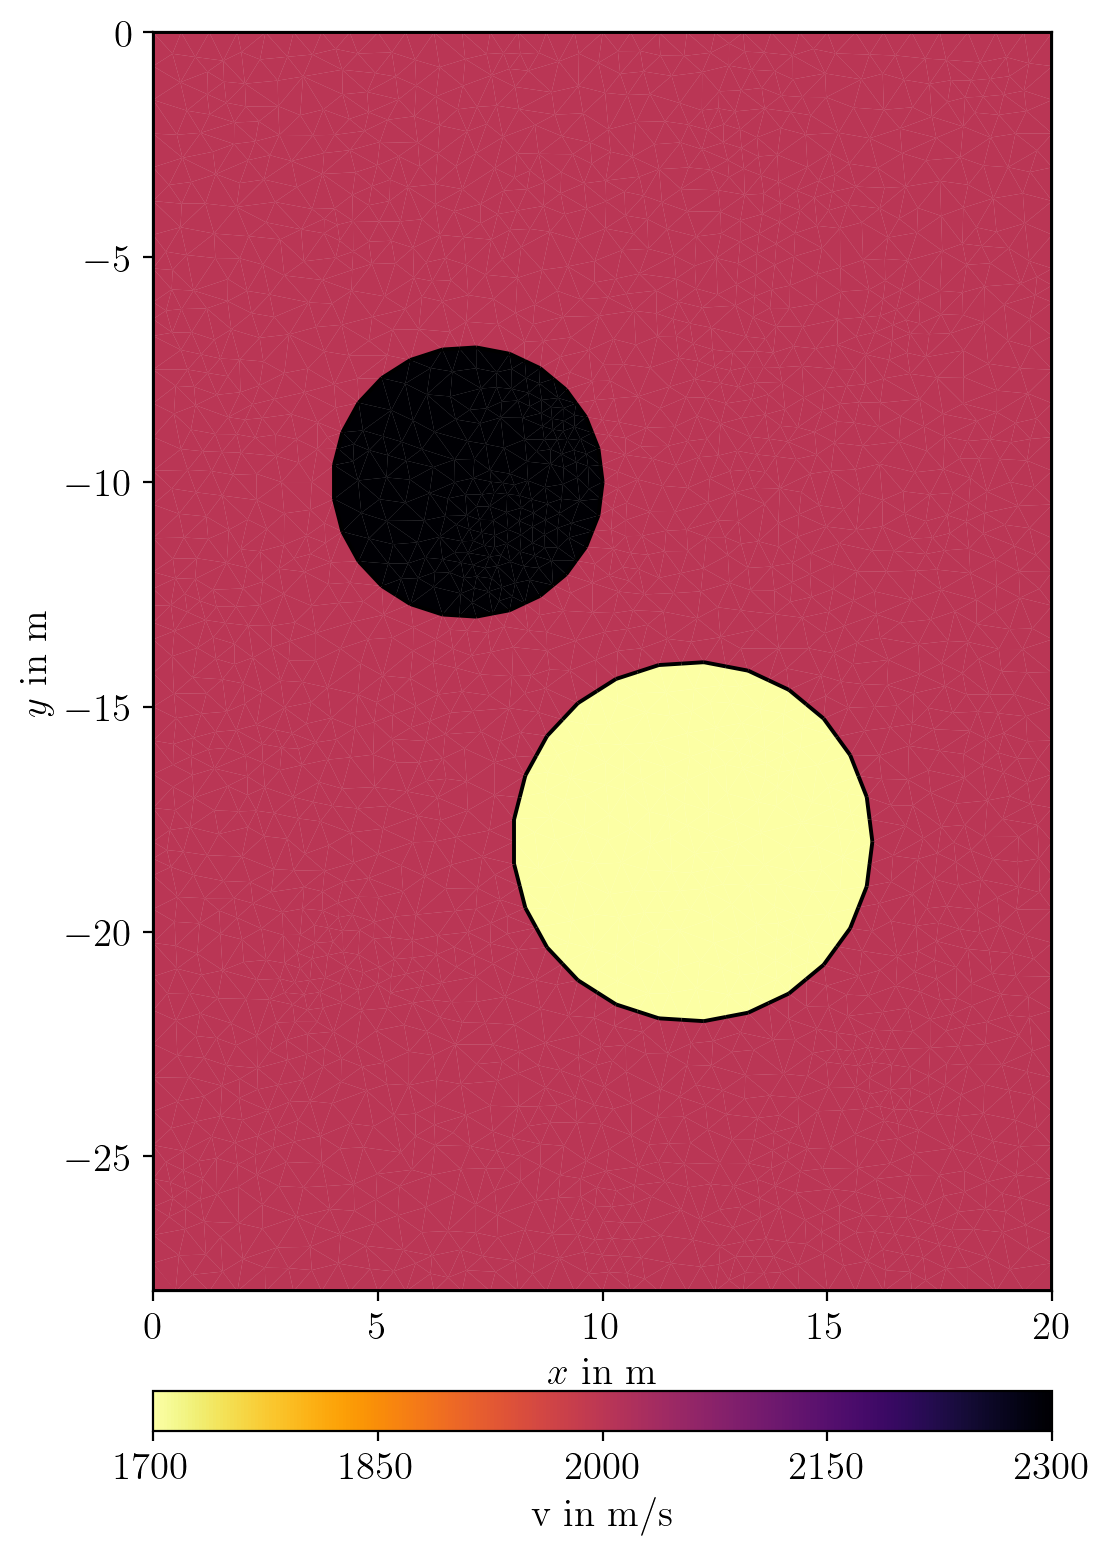
\includegraphics[width=\textwidth]{Media/p3/15.png}
\end{minipage}
\hfill
\begin{minipage}[t]{0.48\textwidth}
    \centering
    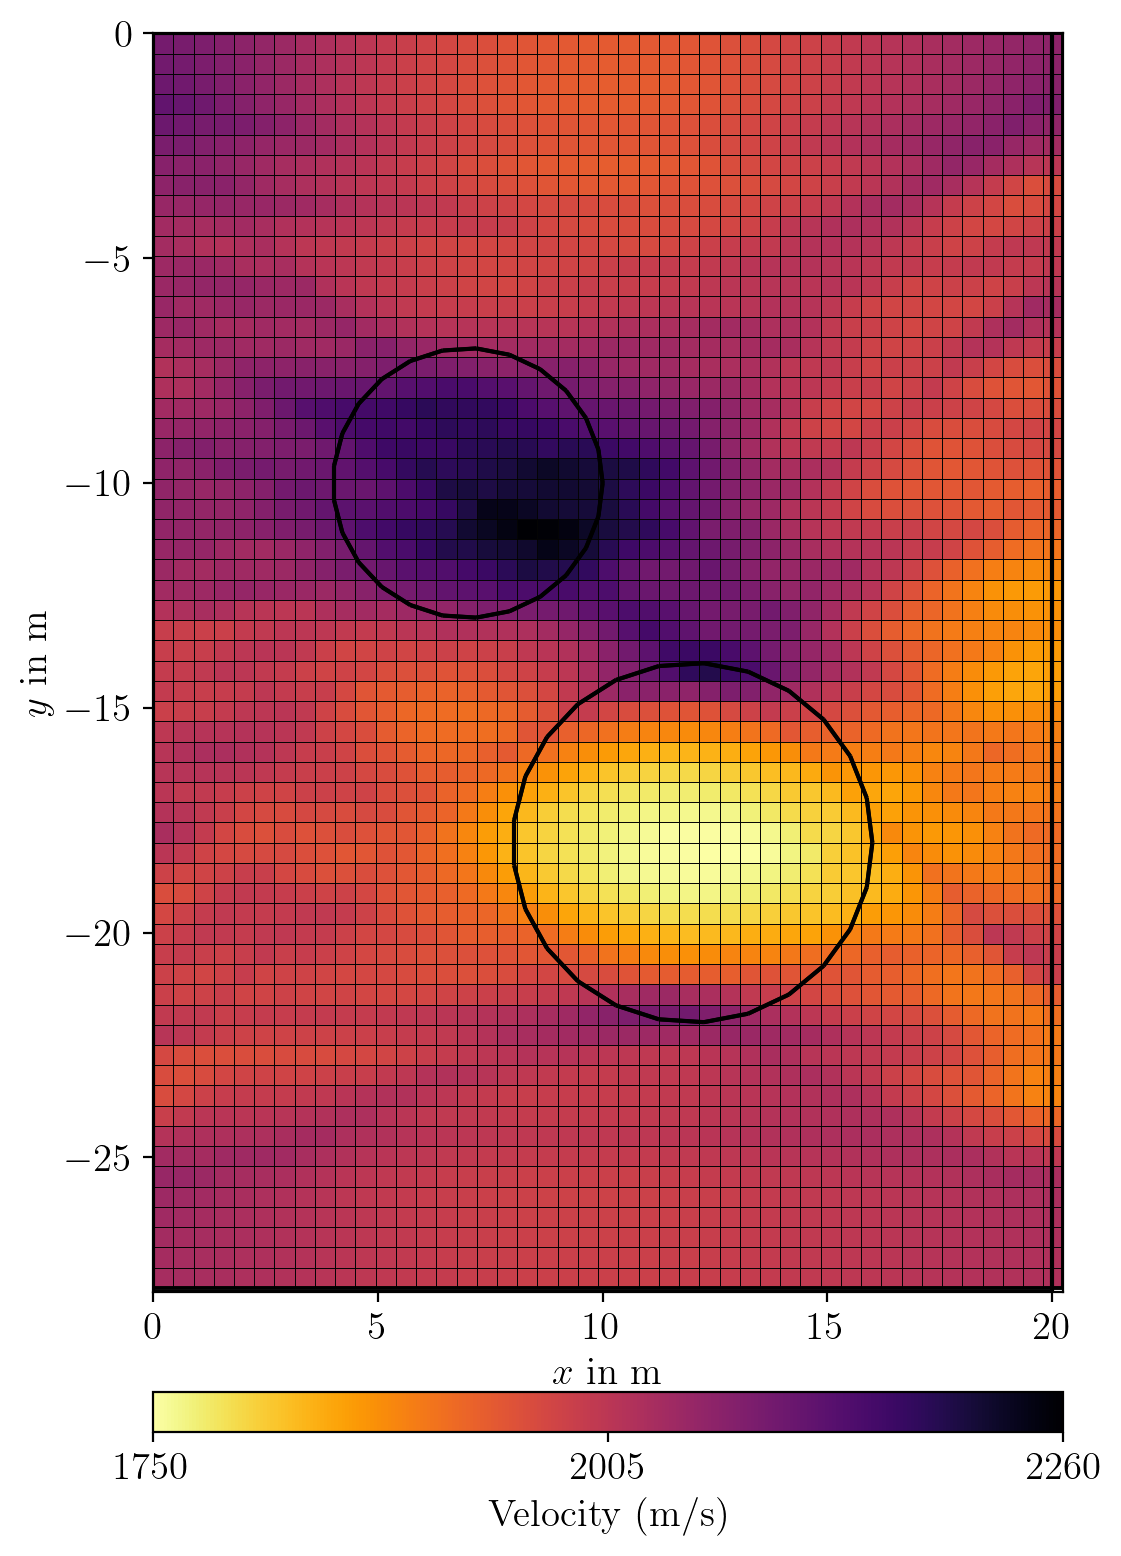
\includegraphics[width=\textwidth]{Media/p3/19.png}
\end{minipage}
\caption{(a.) True velocity model. (b.) Inverted velocity model from the inversion on structured grid. Anomalies are recovered with expected smoothing due to regularization; the low-velocity zone is clearly visible on the left, high-velocity anomaly on the right, with background correctly identified in the central region.}
\end{figure}

\begin{figure}[H]
\centering
\begin{minipage}[t]{0.48\textwidth}
    \centering
    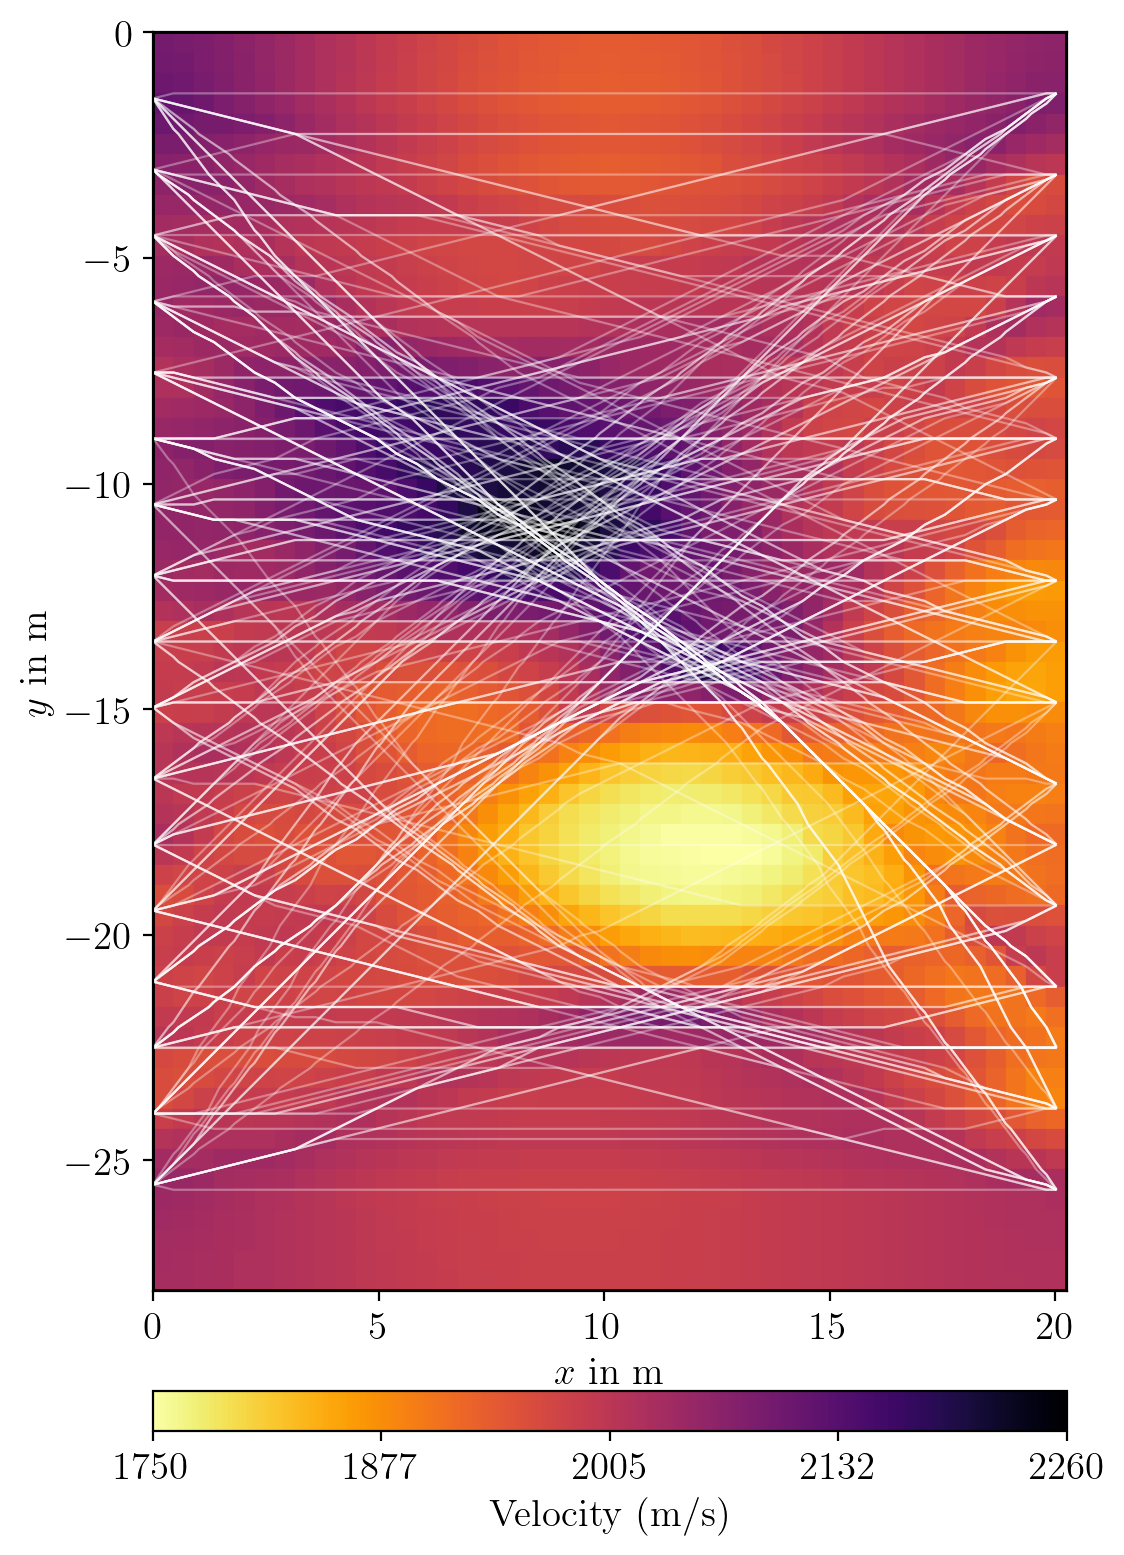
\includegraphics[width=\textwidth]{Media/p3/20.png}
\end{minipage}
\hfill
\begin{minipage}[t]{0.48\textwidth}
    \centering
    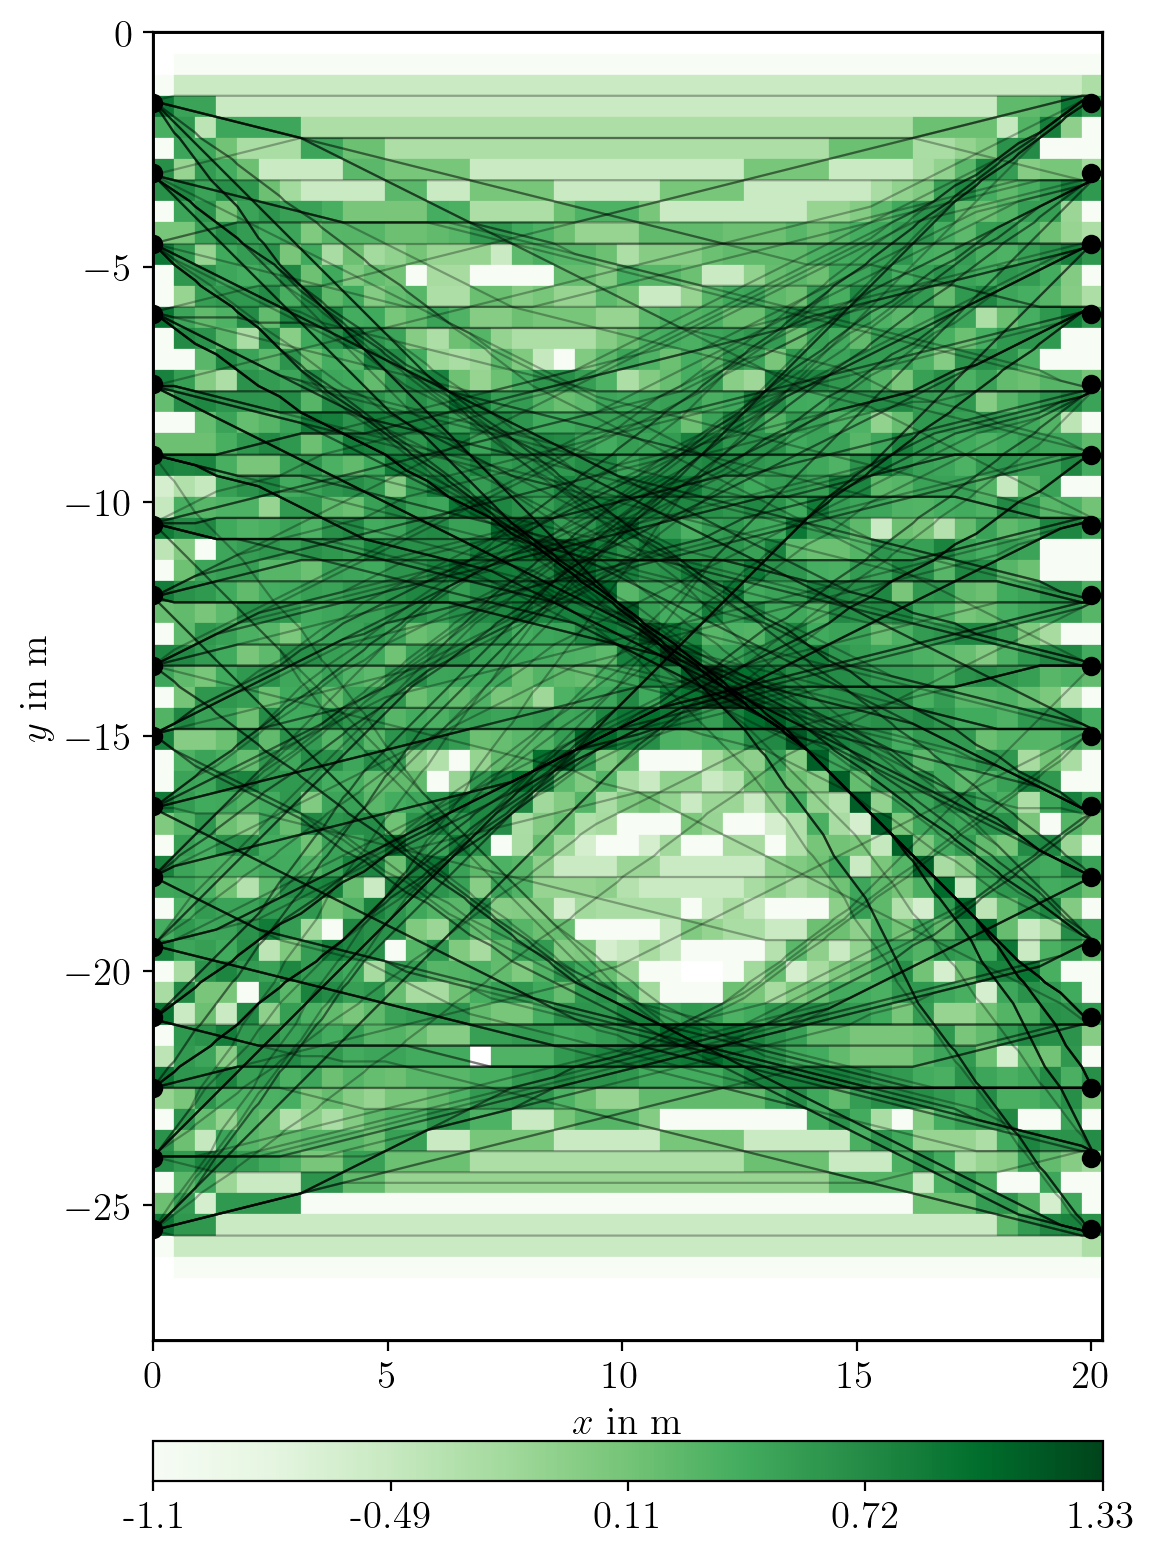
\includegraphics[width=\textwidth]{Media/p3/21.png}
\end{minipage}
\caption{(a.) Ray paths over the recovered model. (b.) Ray coverage map showing cumulative ray-path lengths through each model cell. Note how the rays are attracted by the high velocity anomaly while circumventing the low-velocity region.}
\end{figure}

\section*{Conclusions}
Travel-time tomography via Dijkstra ray tracing and Gauss-Newton inversion is a mature, effective method for near-surface velocity reconstruction. The combination of physical simplicity (ray paths on a mesh), mathematical robustness (well-posed inverse problem with regularization), and computational efficiency ($O(n \log n)$ forward solves) makes it ideal for practical applications. PyGIMLi provides a high-level, user-friendly implementation enabling reproducible workflows from raw data to interpreted models in a few lines of code.

\bigskip
\hrule